% -*- mode: latex; eval: (flyspell-mode 1) -*-
\documentclass[11pt,a4paper]{scrartcl}

\usepackage{minted}
\usepackage{hyperref}
\usepackage{graphicx}
\usepackage{xcolor}
\usepackage{framed}
\usepackage{gensymb}
\usepackage{cmbright}
%\usepackage{newcent} % thos one is good
%\usepackage{mathpazo} % inot as good as charter
%\usepackage{charter} % works quite good
%\usepackage[urw-garamond]{mathdesign} %
%\usepackage[garamond]{mathdesign} %
%\usepackage{ebgaramond} % 
%\usepackage[bitstream-charter]{mathdesign}

%\usepackage{gentium} % looks very good
%\usepackage{sourcecodepro} % 
\usepackage{lmodern}
\usepackage[T1]{fontenc}
\usepackage{makeidx}

\makeindex

\newenvironment{warning}{\begin{framed}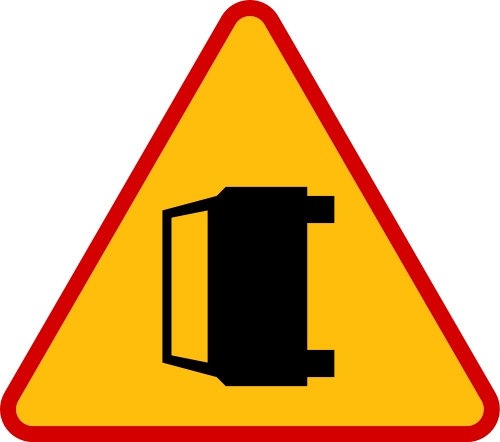
\includegraphics[width=5em]{accident-area-ahead.png}
}{\end{framed}}


\begin{document}

\title{Tutorial for the MOONS FPU grid driver Python library
  module} \subtitle{For driver version 0.7
  .2 (document version \texttt{\input{../git_version}})}

\author{Johannes Nix}

\maketitle

\tableofcontents


\section{Introduction}
\subsection{Related documents}

\begin{tabular}{|ll|}
  \hline
\verb+[1] VLT-TRE-MON-14620-1018+, &  FPU Verification Requirements \\
\verb+[2] VLT-TRE-MON-14620-3017+, & MOONS Fibre Positioner Verification Software Design \\
\verb+[3] VLT-TRE-MON-14620-3016+, & Fibre Positioner Communication Protocol\\
\hline
\end{tabular}


\subsection{Purpose of this document}
This document describes the Python programming interface for the MOONS
Fibre Positioner Unit CAN level driver module.

The CAN level driver allows to control and move Fibre Positioner Units
(FPU) in the MOONS FPU grid by a software interface. This programming
interface is implemented in C++. It is designed to be used in several
different contexts: Primarily, for simultaneously controlling more
than 1000 FPUs in the final MOONS astronomic instrument. Important
secondary uses are verifying and calibrating the components of the
positioning system, developing and testing of algorithms for complex
higher layers of the instrument control system, and engineering and
development of related systems and verification software such as image
analysis.

Using the final verification software will not require the users to
know how to program Python.  However, several parts of the
verification software system and the instrument control software are
entirely or initially developed and tested in Python.  The Python
driver library documented here has the function to make the
functionality of the CAN level C++ driver accessible from Python. As
such, the goal of this document is to describe a toolbox which can be
used to manipulate and test the FPUs as easily as possible, while the
verification software is being developed. The underlying hardware
protocol will only be exposed as much as necessary to understand the
possible states of the hardware.



\subsection{Required knowledge}
\index{Python!introduction}
\index{Python!further information}

It is assumed that the reader has basic knowledge of Python, or,
alternatively, a similar object-oriented language, like Java or C\#.
In the case that using Python scripts is new to the reader, it is
probably helpful to consult the tutorial for Python 2.7 at
\url{https://docs.python.org/2.7/tutorial/}.  Both the current version
of the driver as well as this document use Python 2.7. Python 2, which
is reaching its end of life in 2020, has some differences to Python
3. However this description will proceed in a way that differences to
Python 3 are minimised.

\index{git!further information}
\index{git!getting or updating a repository}
Also, in order to retrieve the current version of the library, the
user needs to have a minimum knowledge of the git version control
system. This is explained, for example, in
``\href{https://git-scm.com/book/en/v2/Git-Basics-Getting-a-Git-Repository}{getting
  a git repository}\footnote{https://git-scm.com/book/en/v2/Git-Basics-Getting-a-Git-Repository}''.

\section{Setting up the library module}
\index{driver!building}

This section deals with retrieving, installing and configuring the
driver module. On the MOONS workstation, it can be skipped because the
FPU driver is already installed.  In this case, you can proceed
directly with section~\ref{sec:minimalexample} on
page~\pageref{sec:minimalexample}.

\subsection{Getting the source code}

To set up the library module, it is first
necessary to retrieve a current copy of its source code.
On the moons-pc01 workstation, this can be done using the
command \mint{bash}|git clone /home/jnix/fpu_driver|
This creates a new directory with the name \texttt{fpu\_driver}
and populates it with the source code.

Alternatively, a fresh copy can be retrieved from the UKATC dalriada
server. Doing this this requires a personal user account on that
server. Assuming the account name is \texttt{carl}, this is done by
the command
\index{git!repository setup}

\mint{bash}|git clone carl@dalriada/sw/sw4/jnix/MOONS/fpu_driver|

After entering the password for user \texttt{carl}, the
source code is copied into the new folder \texttt{fpu\_driver}.

\subsection{Refreshing the source code}
\index{driver!building!update or change version}
To refresh the source code, change the
working directory to \texttt{fpu\_driver},
and issue the command

\mint{bash}|git pull|


\subsection{Building specific revisions}
\index{git!get specific version}
\index{driver!building!specific version}
In the default case, the library is build from
the master branch of the git repository.
The master branch contains the most current
working version.
In some cases, it might be required to
use a specific revision of the library.
Assuming that we need, as an example,
to build version v0.5.2 of the library,
checking out this revision is done with the
command

\mint{bash}|git checkout v0.5.2|

After this, one can proceed with building the library as normal. To
switch back to the master branch, issue the command

\mint{bash}|git checkout master|


\subsection{Building the library module}
\index{driver!building}
To build the Python library module,
change the working directory to \texttt{fpu\_driver},
and issue the command \mint{bash}|make pyext|

In order for this to work, the required dependencies need to be
installed. For the MOONS workstation, this is always the case. To
install these dependencies on other computers, follow the detailed
instructions in the appendix section~\ref{sec:installationfromscratch}
on page~\pageref{sec:installationfromscratch}.  A more concise summary
is given in the text file ``\texttt{doc/INSTALL}''.

\subsection{Enabling debug output of CAN messages}

Previous versions of the driver required to change macros in the C
source code to enable low-level logging of CAN commands.  With driver
version 0.5.3, a comprehensive log of sent and received CAN messages
is enabled by default. See section~\ref{sec:logging} on
page~/\pageref{sec:logging} for the location of these logs, and any
further details.


\subsection{Environment configuration}
\index{driver!configuration}
\index{setup!environment variables}
\index{environment variables}
For the Python module to work, the directory \texttt{/user/local/lib}
needs to be added to the environment variable
\texttt{LD\_LIBRARY\_PATH}.

Also, it is probably useful to add the \texttt{python} directory and
the current directory to the environment variable \texttt{PYTHONPATH},
so that the driver module can be found independently from the current
working directory.  Assuming a standard Ubuntu or Debian setup, this
can be done by adding the following lines to the file \texttt{.bashrc}
in the user-specific home directory:

\begin{minted}{bash}
  export LD_LIBRARY_PATH=$LD_LIBRARY_PATH:/usr/local/lib
  export PYTHONPATH=$PYTHONPATH:$HOME/fpu_driver/python:.
\end{minted}
 
Further, it is recommended to set the default log directory to point
to a file system which has a lot of free space, for example:
\begin{minted}{bash}
  export FPU_DRIVER_DEFAULT_LOGDIR=/moonsdata/logfiles
\end{minted}


\subsection{Hardware configuration and addressing}
\index{addressing!FPUs}
\index{indexing FPUs}
\index{FPU IDs!configuration}
\index{CAN ID}
\index{FPU!addressing}
\index{FPU!hardware configuration}
\index{networking!FPU addressing}
Messages to an individual FPU are sent using a logical number, the FPU
ID, which starts at 0 and goes up to a maximum value.

The messages from the driver to FPUs are transported by two layers of
hardware.

\index{EtherCAN gateway!configuration} \index{IP address!of EtherCAN
  connection} \index{port number!of EtherCAN connection} First, the
messages are transmitted by an Ethernet socket connection to up to
three EtherCAN gateways. To connect to each gateway, its IP address
and port number are used. The default IP number, to which the EtherCAN
gateway card is configured, is "\texttt{192.168.0.10}", and the
connection uses port 4700 by default. In this case, the EtherCAN
gateway (or if several are used, all of them) needs to be connected to
a private network interface to which IP packets to network
\texttt{192.168.0.0/24} are routed.

From the selected gateway, the messages are then forwarded to up to
five CAN buses. Each bus connected to a gateway is identified with a
number as well, and is connected to up to 72 (currently, 67) FPUs.
\index{DIP switch} To identify each FPU in a setup with many FPUs,
they have to use a CAN ID which is unique on each bus, ans is
different from zero. This ID is physically configured by manually
toggling a DIP switch in the FPU's electronics board. The current
driver uses a fixed continuous mapping (basically, array indexing)
from the translation of FPU IDs to gateway number, bus number, and CAN
ID\footnote{Future versions of the software will relax this
  restriction}.

This results in that each FPU has a physical address with three
elements: gateway number, bus number, and CAN ID.

\emph{For addressing a single FPU, this simply means that its CAN ID
  needs to be set to one, which means its DIP switch needs to be set
  to the delivered configuration. That FPU then needs to be connected
  to the first bus on the first gateway}.


\subsection{Software protection flag}
\index{hardware protection}
\index{soft\_protection flag}
The FPU control chain uses a layered approach to make sure that fibre
positioner units do not get damaged.  At the bottom layer, there is an
electronic collision protection, which will switch off the motors and
send a warning message if two FPUs touch each other. This protection
level is called ``hardware protection''.

\index{wear and tear} \index{avoiding hardware damage} \index{hardware
  protection} However, even if a direct damage should be avoided by
this protection, activating it involves that the motors are suddenly
stopped, which decreases the precision and can significantly increase
wear and tear, thus reducing the life time of the stopped
FPU. Therefore, the hardware protection should be used only at an
emergency level. Furthermore, the hardware protection does not cover
all situations.

For these two reasons, the driver software performs a number of
additional checks which should ideally ensure that no collisions
occur. These checks are performed every time an FPU is moved, or
configured to move, and are named ``software protection''.

In some situations, specifically if the hardware protection needs to
be tested, it can be necessary to switch off and deactivate this
protection. This can be done using the ``\texttt{soft\_protection}''
keyword argument. Passing the value
``\texttt{soft\_protection=False}'' will switch the software
protection check off.



\subsection{Communication protocol versions}
\index{protocol!see{CAN protocol}} \index{CAN protocol versions}
\index{CAN protocol versions! version 1 capabilities} The FPU driver
sends commands to the fibre positioner units, which use a specific
communication protocol. This protocol needs to match the FPUs firmware
and its capabilities. The current version of the driver (version
0.6.x) uses ``communication protocol version 1'', which has some
restrictions in functionality.

A significant difference in the hardware protection capabilities is
that cases in which the alpha arm of the FPU hits the limit switch
need to be manually recovered from. This is explained in
section~\ref{sec:recovery} on page~\pageref{sec:recovery}.


\begin{warning}
  \textbf{WARNING: Before first issuing a \texttt{findDatum()}
    command, make sure that both the datum switch and the alpha limit
    switch work. A defective or incorrectly wired alpha limit switch
    will cause the datum command to damage the hardware. The software
    cannot protect against this.}
\end{warning}


\begin{warning}
\textbf{WARNING: Never issue a \texttt{findDatum()} command when the
  alpha arm is in a limit breach position (on the other side of the
  limit switch). No hardware protection is active in this state.}.
\end{warning}

Another important point, is that when doing a first manual datum
search after powering on an FPU , it is important to make sure that
the instructed search direction will move the beta arm to the datum
position. The current version of the driver software does not allow
any more to do a datum search of an uninitialised FPU without
explicitly passing the required search direction.

If the wrong direction is passed, this will cause a collision.  This
incurs the risk to destroy the FPU if the collision detection is not
verified to be working for this unit.  Otherwise, running into a
collision is still highly undesirable because the lifetime and
precision of the FPU will be reduced.

\begin{warning}
  \textbf{WARNING: When using a manual \texttt{findDatum()} command,
    make sure that the beta arm is moving into the right direction, to
    avoid any collisions!}
\end{warning}


\index{datum search!independent operation of alpha and beta arms} The
FPU verification system requires the additional capability to datum
the alpha and beta arms separately.  This is supported by driver
versions equal or newer than 0.5.2 and a firmware that supports the
CAN protocol version 1.1 or later. Earlier firmware versions do not
support this mode of operation.



\section{A minimal example}
\label{sec:minimalexample}
\index{example script}\index{movements!example}
\index{connect()!example}
\index{driver!initialisation!example}
\index{getGridState()!example}
\index{gen\_wf()!example}
\index{configMotion()!example}
\index{executeMotion()!example}
\index{findDatum()!example}
\index{version information!retrieving!example}
The following listing shows a minimal example of the
driver usage, and explains the underlying concepts
step by step.

Importantly, the example assumes that the FPUs have been powered on
before, and have already performed an initial datum search.
Section~\ref{sec:initialsearch} and ~\ref{sec:refinitialsearch} give
more information about how to do this.

\index{waveforms!example}
\index{driver!initialisation!example}
\index{getGridState()!example}
\begin{minted}[linenos]{python}

from __future__ import print_function
import FpuGridDriver
from FpuGridDriver import TEST_GATEWAY_ADRESS_LIST as gw_address
from fpu_commands import list_positions, list_angles, \
       list_deviations, list_states, gen_wf
# print the driver version, just to check
print("The FPU driver version is:", FpuGridDriver.__version__,
      ", CAN PROTOCOL version:", FpuGridDriver.CAN_PROTOCOL_VERSION)

NUM_FPUS = 1 # set number of FPUs to 1
gd = FpuGridDriver.GridDriver(NUM_FPUS)
# connect to gateway with default IP 192.168.0.10
print("connecting grid:", gd.connect(address_list=gw_address))

print("getting grid state:")
grid_state = gd.getGridState()


print("issuing findDatum:")
gd.findDatum(grid_state)
print("findDatum finished")

# We use grid_state to display the starting position
print("the starting position (in degrees) is:",
       list_angles(grid_state))

# Generate a waveform which moves the alpha arm by +45
# degree, and the beta arm by +15 degree. 

alpha_move = 45
beta_move = 15

# Generate the required waveform for one FPU
waveform = gen_wf(alpha_move, beta_move)

# upload the waveform to the FPU
gd.configMotion(waveform, grid_state)

# start the movement
print("starting movement by (45,15) degree")
gd.executeMotion(grid_state)

print("the reached position (in degrees) is:",
       list_angles(grid_state))

print("ready")

\end{minted}


\subsection{Import statements}
\index{import statements}

The import statements in lines 1 -- 4 load the following modules and
configurations:

\begin{itemize}
\item In line 1, the print function and the division operator is
  configured to work as in Python 3.
  
\item ``\texttt{import FpuGridDriver}'' in line 2 loads the driver
  library module. (If this import command fails, check that both
  \verb+LD_LIBRARY_PATH+ and \verb+PYTHONPATH+ have the right values.)

  \index{gateway!configuration}
  \index{IP address!of EtherCAN gateway}
\item The line ``\texttt{from FpuGridDriver import
  TEST\_GATEWAY\_ADRESS\_LIST}'' loads a default address which refers to
  the EtherCAN gateway which is used. This address would be different
  when one wants to select a different gateway. The default
  address used by the EtherCAN gateway card is 192.168.0.10,
  and the card must be connected to a private (internal) network.

\item The line ``\texttt{from fpu\_commands import \ldots}'' imports a
  few utility commands which help to display positions and to generate
  movement waveforms.

 
\end{itemize}

\subsection{Grid driver object}
\index{driver!instantiation}

In line 10 of the example script, the used number of FPUs is set to
one, and in line 11, the FPU grid driver is initialised with that
value. The returned object, which is referenced by the Python variable
``\texttt{gd}'', is always required to access the FPUs.

\subsection{Driver methods}
\index{networking!see{also connect()}}
\index{connect()}
\index{driver!how to call methods}
The driver object allows to invoke method calls (methods are also
often called member functions) which control the FPU hardware. The
method names always start with a dot after the name of the driver
object.  So, \texttt{gd.abc()} would call method ``abc'' of the driver
object. Like normal function calls, they usually have parameters.

In this case, the method \texttt{connect()} connects the driver to one
or more EtherCAN gateways and starts listening to messages from the
FPUs. The parameter \texttt{gw\_address} defines to \emph{which}
gateways the driver listens to. Section~\ref{sec:connect}
on~\pageref{sec:connect} explains the default parameters which are
used.

As can be seen in the example, the methods have return values.  In
case of serious errors, the methods raise a Python exception. The
Python program does not need to explicitly disconnect and
de-initialise the driver, this happens automatically when the program
terminates\footnote{However if required, you can use the statements
  \texttt{gd.disconnect()} and \texttt{del gd}, which disconnects and
  deletes the driver object.}.



\subsection{Grid state variable}
\index{grid\_state!introduction} Almost all commands to the driver
receive and return a snapshot of the current state of the used FPU
(or, if there are several, of all FPUs). That snapshot is passed in a
variable called \texttt{grid\_state}. This variable contains all the
information a user might need about the state of the FPUs - their
current positions, which commands they will accept right now, whether
there are any collisions, whether the step counters have been zeroed,
whether a limit switch was hit, and so on. With each invocation of a
method, the old grid state is passed as a reference parameter, and its
new value is returned in the same variable.

To retrieve the current grid state information, the method
``getGridState()'' is used, as is done in line 16. In our listing, the
grid state data is assigned to the variable named
\texttt{grid\_state}.  The \texttt{getGridState()} function always
returns immediately, as it just takes a snapshot of the state
data. Because \texttt{grid\_state} is used so frequently, a short-hand
alternative name which many of the example scripts use is the name
\texttt{gs}.  Technically, these names are simply Python variable
names, which can be arbitrarily chosen by the user.

\subsection{Moving the FPU around}
\index{movements!example}
\index{movements!overview}
The example script then proceeds to use three methods to move
the FPUs:

\begin{description}
\item[\texttt{findDatum()}] in line 20 moves the FPU to the datum
  position. After this, the internal step counters are set to zero,
  both for the alpha and for the beta arm.

  Keep in mind that this requires both the alpha arm to be in a safe
  positions -- the alpha arm must be inside its operating range (it
  must not have passed the limit switch). If the software needs
  additional information to perform a safe datum search, an automatic
  search is not possible, and a \texttt{DE\_PROTECTION\_ERROR}
  exception is returned. How to do a manual datum search is described
  in the next section (section~\ref{sec:initialsearch}).

  \index{waveforms!configuring}
\item[\texttt{configMotion()}] is a method which sends a table with
  movement instructions, also called ``waveform table'', to the
  FPU. In the listing, this is done in line 37. The waveform table is
  stored in the variable \texttt{waveform}, which is defined in line
  34.

\item[\texttt{executeMotion()}] in line 41 is the command which starts
  the movement of the FPU. This command returns when the movement is
  complete and the FPUs have stopped to move. In case of an error, the
  command generates a Python exception.

\end{description}

\subsection{Utility functions}
\index{list\_angles()!example}
\index{list\_positions()!example}
\index{gen\_wf()!example}
The example also shows two utility functions for generating movement
data, and displaying information about the FPU state:

\begin{description}
\item[\texttt{list\_angles()}] is a function which takes a \texttt{grid\_state}
  variable, and displays the approximate positions of the FPUs as
  alpha and beta angles, in degree units.

\item[\texttt{gen\_wf()}] is a function which takes an (alpha,beta)
  pair of angle values, scaled in degrees, and generates a valid
  waveform which can be send to the FPU.  The waveform which is passed
  is a regular Python data structure and can be displayed and
  manipulated like any other Python object.  The user only needs to
  take care that it contains valid movement data when it is passed to
  the \texttt{configMotion()} method!


\end{description}


\subsection{Initial datum search}
\label{sec:initialsearch}
\index{datum search!initial} \index{DE\_PROTECTION\_ERROR} As
mentioned above, the listed example relies on the fact that the FPUs
already have been powered on, and a successful datum search was
performed before. Based on a valid datum search, the FPU firmware can
decide in which direction the beta arm can be moved. This mode of
operation is called ``automatic'' datum search.

However, when an FPU was just powered on, it lacks this information,
so it cannot perform an automatic search. In this case, attempting to
start an automatic datum search would result in a
\texttt{DE\_PROTECTION\_ERROR} exception. Instead, the operator needs
to instruct the hardware in which direction it must move. This is done
by passing additional parameters to the \texttt{findDatum()} command,
like this:


\begin{minted}{python}
  gd.findDatum(grid_state, search_modes={0 : SEARCH_CLOCKWISE,
               1: SEARCH_ANTI_CLOCKWISE, 2 : SEARCH_CLOCKWISE},
               soft_protection=False)
\end{minted}

Here, the integer numbers (0, 1, 2, \ldots) correspond to FPU numbers,
and the symbols \texttt{SEARCH\_CLOCKWISE} and
\texttt{SEARCH\_ANTI\_CLOCKWISE} instruct this FPU in which direction
it should move. These symbols needs to be imported by an ``import''
statement from the \texttt{FpuGridDriver} module.  Here, ``clockwise''
and ``anti-clockwise'' refer to the directions when looking from
above. FPUs which do not get such an instruction will not move. 


When the FPUs were actually initialised before, it is possible to use
the ``automatic'' mode of the \texttt{findDatum()} command, by passing
the \texttt{soft\_protection} flag without a direction specification.

\index{safety!datum operation}
\begin{warning}
  \textbf{WARNING: When doing a manually directed datum search, always
    double-check that the beta arm will correctly move to the datum
    position with the given direction. Otherwise, the command will
    cause a collision, leading to increased wear and tear, or even to
    hardware damage.}
\end{warning}


\subsection{Interactive inspection of the FPU state}
\index{fpu\_state!interactive inspection}
\index{fpu\_state|see{~\emph{also} FPU state}}
\index{Python!running interactively}
\index{driver!configuration!example}
\index{collisions!indicator flags}
\index{grid state!interactive inspection}
\index{FPU!detailed state information}
\index{FPU!state!inspecting details}
\index{FPU!state!of grid|see{\emph{also} grid state}}
\index{state|see{FPU state}}
\index{position information!details}
\index{position information!retrieval}
\index{grid state!position|see{position information}}
\index{grid state!datum flags}
\index{datum search!flag inspection}
\label{sec:fpustate}
The grid state variable holds a large amount of detail information
about the current state of FPUs. This is by design, because upper
layers of the software need to be able to deal with complex scenarios
such as collisions, or even a pile-up of many collided FPUs, and
correct them. However, only a part of this information is required by
the verification system.

When trying to diagnose and understand errors, it is often helpful to
access this state information in an interactive way.  To do this, we
will make use of Python's capability to run any commands which appear
in a script equally well when entered interactively. In addition, the
Python interpreter can be started with the ``-i'' (interactive) option
which has the effect that after after all commands in a script have
been executed, or after any exception has been thrown, the interpreter
opens a command line or ``read-eval-print-loop'' in which commands can
be entered and executed in the interactive mode. Every time when a
typed-in expression or function call returns a value, the value is
printed out before the command prompt appears again.

For example, let's assume that the script on
page~\pageref{sec:minimalexample} is shortened to the first 36 lines
and stored to a file named \texttt{short\_script.py}. We then might
run the following interactive session (where the lines starting with
``\texttt{\$}'' and ``\verb+>>>+'' are interactive input, and
everything else is output):



\begin{minted}{python}
$ python -i short_script.py
initializing driver:  DE_OK
connecting grid: DE_OK
getting grid state:
issuing findDatum:
findDatum finished
the starting position (in degrees) is: [(0.0, 0.0)]
>>> grid_state.FPU[0]
{ 'last_updated' : 61604074.942,  'pending_command_set' : 0,
  'state' : 'READY_FORWARD',  'last_command' : 9,  'last_status' : 0,
  'alpha_steps' : 0,  'beta_steps' : 0,
  'alpha_deviation' : 0,  'beta_deviation' : 0,
  'timeout_count' : 0,  'step_timing_errcount' : 0,
  'direction_alpha' : 0,  'direction_beta' : 0,
  'num_waveform_segments' : 0,  'num_active_timeouts' : 0,
  'sequence_number' : 0,  'ping_ok' : 1,  'movement_complete' : 0,
  'alpha_was_zeroed' : 1,  'beta_was_zeroed' : 1,
  'is_locked' : 0,  'alpha_datum_switch_active' : 0,
  'beta_datum_switch_active' : 0,
  'at_alpha_limit' : 0,  'beta_collision' : 0,
  'waveform_valid' : 1,  'waveform_ready' : 1,  'waveform_reversed' : 0,
  'register_address' : 0,  'register_value' : 0x1,
  'firmware_version' : 1.3.0,  'firmware_date' : '0-0-0',
  'serial_number' : "102",  }
>>> list_angles(grid_state)
[(-181.0, 0.0)]
>>> gd.executeMotion(grid_state)
fpu_driver.E_DriverErrCode.DE_OK
>>> grid_state.FPU[0]
{ 'last_updated' : 61604357.008,
  'pending_command_set' : 0,
  'state' : 'RESTING',  'last_command' : 7,  'last_status' : 0,
  'alpha_steps' : 5125,  'beta_steps' : 1264,
  'alpha_deviation' : 0,  'beta_deviation' : 0,
  'timeout_count' : 0,  'step_timing_errcount' : 0,
  'direction_alpha' : 0,  'direction_beta' : 0,
  'num_waveform_segments' : 0,  'num_active_timeouts' : 0,
  'sequence_number' : 0,  'ping_ok' : 1,
  'movement_complete' : 1,
  'alpha_was_zeroed' : 1,  'beta_was_zeroed' : 1,
  'is_locked' : 0,  'alpha_datum_switch_active' : 0,
  'beta_datum_switch_active' : 0,
  'at_alpha_limit' : 0,  'beta_collision' : 0,
  'waveform_valid' : 1,  'waveform_ready' : 0,
  'waveform_reversed' : 0,
  'register_address' : 0,  'register_value' : 0x1,
  'firmware_version' : 1.3.0,  'firmware_date' : '0-0-0',
  'serial_number' : "102",  }

>>> list_angles(grid_state)
>>> list_angles(gs)
[(-136.00385502825844, 14.991475555234816), ]
>>>
\end{minted}

In this listing, entering the expression \verb+grid_state.FPU[0]+
displays the state parameters of FPU 0 (which is the only one we have
because \texttt{NUM\_FPUS} was set to 1).

\begin{sloppypar}
Just to pin-point two of the more important bits of information, the
fields ``\texttt{alpha\_steps}'' and ``\texttt{beta\_steps}'' contain
the current step counts of an FPU, and the fields
``\texttt{alpha\_datum\_switch\_active}'' and
``\texttt{beta\_datum\_switch\_active}'' contain the current position
of the datum switches. The field ``\texttt{state}'' contains the
current state of the FPU, ``\texttt{firmware\_version}'' contains the
version of the FPU firmware, and ``\texttt{serial\_number}'' the serial
number of the FPU, if it was stored in the firmware. One can see that
after issuing the \texttt{executeMotion} command, the state of the FPU
changes from \texttt{READY\_FORWARD} to \texttt{RESTING}. Actually,
the output of the \texttt{list\_angles()} utility function mentioned
before is normally (that is, if at least one datum search was
completed) just a scaled version of the ``alpha\_steps'' and
``beta\_steps'' fields. The flags \texttt{alpha\_was\_zeroed} and
\texttt{beta\_was\_zeroed} are set to \texttt{True} when the datum
position was reached at least once since the driver was started, and
no collisions, limit switch breaches, or abortMotion commands have
happened since.
\end{sloppypar}

\subsubsection*{Capturing interactive output}
\index{capturing output} \index{troubleshooting!capturing output} To
investigate and communicate any difficulties or errors, it is
sometimes helpful to capture the interactive output. A helpful tool
for this is the Linux ``\texttt{script}'' command, which does exactly
this, and is installed on the MOONS workstation.  For further
information, please consult the ``script'' man page.



\subsection{FPU states}
\index{state|see{FPU!FSM states}} \index{Finite State
  Machine|see{FPU!FSM states}} \index{FPU!states, how to query}
\index{FPU!FSM states!overview} \index{FPU!FSM states!table}
\index{FPU!FSM states|see{~\emph{also} fpu\_state}} The state of an
FPU is summarised in a enumeration value, which is stored in the
attribute ``\texttt{state}''. For example, the state of FPU 0 can be
retrieved by

\begin{minted}{python}

>>> grid_state.FPU[0].state
\end{minted}


\begin{table}
    \begin{minipage}{0.8\textwidth}
  \begin{centering}
\begin{tabular}{|l|p{0.7\textwidth}|}
  \hline
  \textbf{State name} & \textbf{Description} \\
  \hline 
UNKNOWN & The state of the FPU is not known, the driver needs to
be connected to the EtherCAN gateway first and retrieve the state.\\
\hline
UNINITIALIZED & The FPU has been pinged successfully, but it was
  so far not zeroed to the datum position, so no movements are
  possible.\\
\hline
LOCKED & The FPU was locked, which inhibits movement of this
  FPU.\footnote{This is a facility provided by protocol version 2}\\
\hline
DATUM\_SEARCH & The FPU is currently searching for the datum
position.\\
\hline
AT\_DATUM      & The FPU has reached the datum position.\\
\hline
LOADING & The FPU is currently configuring a new movement waveform.\\
\hline
READY\_FORWARD & The FPU has successfully been configured with a waveform
and is ready to move in the forward
  direction of the waveform table.\\
\hline
READY\_REVERSE& The FPU is ready to move in reverse direction along the
  waveform table.\\
\hline
MOVING        & The FPU is currently moving.\\
\hline
RESTING       & The FPU has finished its movement.\\
\hline
ABORTED & The movement was aborted, either by an internal error
  in the FPU controller, or by an explicit abortMotion command.\\
\hline
OBSTACLE\_ERROR& The FPU has either detected a collision of the
  beta arm, or the alpha arm has hit the limit switch. In both cases, the
  movement was aborted. \\
\hline
\end{tabular}
\end{centering}
\end{minipage}
\caption{List of FPU states and their definitions}
\label{tab:fpustates}
\end{table}

\begin{figure}
\index{FPU!states!allowed transitions}
  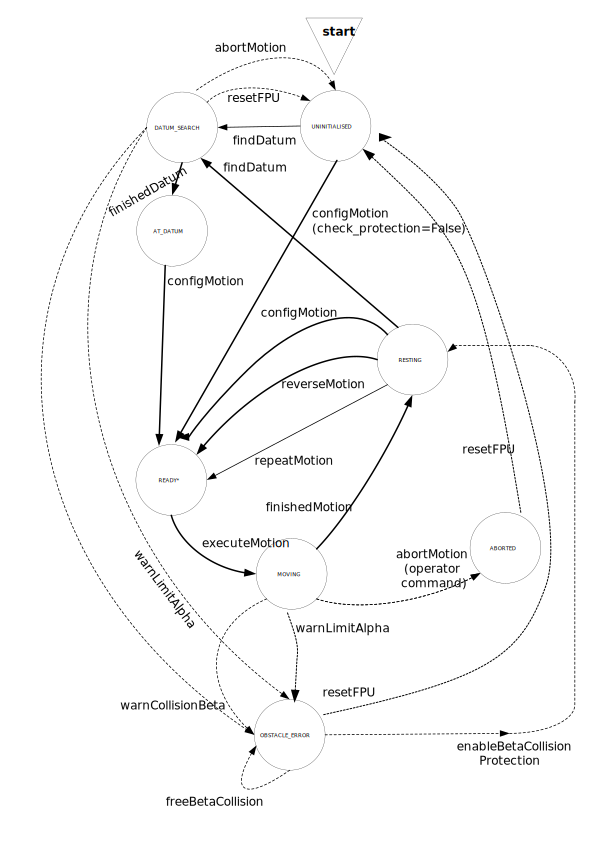
\includegraphics[width=1\textwidth]{FPU-state1.pdf}
  \caption{Allowed state transitions of a single FPU for CAN protocol
    version 1, and the associated driver commands and CAN messages.}
  \label{fig:states}
\end{figure}


Generally, each FPU is always in exactly one of 12 different states.
Changes can be described by the concept of a ``finite state machine'':
Each state allows a number of different commands, and commands can
change the FPU state from the current state into another allowed
state.  Some of the states are visited during any normal operation of
the FPU, and some are reached as a result of errors.
Table~\ref{tab:fpustates} on page~\pageref{tab:fpustates} lists the
different states.


\index{FPU!possible state transitions}
Figure~\ref{fig:states} on page~\pageref{fig:states} shows, as a
reference, the states of the FPU, and the possible state transitions
and commands which are allowed in protocol version 1.


\subsection{Checking the switch states}
\index{alpha limit switch!checking state}
\index{limit switch!check the state}
During initial testing, it is advisable to test the function
of the switches -- especially the alpha limit switch --
without performing a datum operation. The reason for this
is that if the alpha limit switch should not work, the
datum operation would probably damage the FPU irreparably.

To test the switches, the FPU should be driven manually to a position
where the corresponding switch is required to engage. At this point,
the command

\begin{minted}{python}
  gd.getSwitchStates(grid_state, fpuset=[])
\end{minted}

should be used to verify that the switch is working.


\section{Common tasks}

The following sections describe several common tasks
and describes which commands can be used to perform them.


\subsection{Checking the connection}
\index{networking!check}
\index{networking!example}
\index{errors!connection}
\index{connection,checking the}
\index{troubleshooting!connection problems}
\begin{samepage}
At some points, it is of interest what the state of
the connection to the CAN gateway and of the FPUs is.
This can be achieved by the following commands:
\begin{minted}{python}
grid_state = gd.getGridState()
grid_state.driver_state  
\end{minted}
The return value is the connection state of the driver, which is
\texttt{DS\_CONNECTED} if the connection is live.  In the case that the
connection fails, it is still possible to retrieve state information
on the FPUs, but it cannot be refreshed any more until the connection
is re-established using the \texttt{connect()} method of the driver
object.
\end{samepage}

\index{connection errors!example} Of course, it is possible that the
connection between driver and EtherCAN gateway works, but that an FPU
does not respond, for example, if the CAN bus connection wiring is
broken, or the FPU has no power. This can be checked by the commands:

\begin{minted}{python}
  gd.pingFPUs(grid_state)
  grid_state.FPU[0].ping_ok
\end{minted}

In the case that the FPU responds, the returned value is
\texttt{True}.  If the FPU does not respond, the value of the
\verb+ping_ok+ becomes \texttt{False}.

Errors both during making the socket connection, and when sending
commands to the FPUs cause a \texttt{ConnectionFailure} exception to
be thrown, like in this log file:

\index{exceptions!example}
\begin{minted}{python}
  $ python -i test_mockup/test_asyncMotion.py 
connect: Connection refused
Traceback (most recent call last):
  File "test_mockup/test_asyncMotion.py", line 12, in <module>
    print("connecting grid:", gd.connect())
  File "/sw/sw4/jnix/MOONS/fpu_driver/python/FpuGridDriver.py", line 65, in connect
    return self._gd.connect(address_list)
    fpu_driver.ConnectionFailure: DE_NO_CONNECTION: The FPU Driver
    is not connected to a gateway.
>>> 
\end{minted}


The associated error message and enumeration symbol should be
sufficient to determine the cause of the problem. A comprehensive list
of exceptions and error codes is given in section~\ref{sec:errors} on
page~\pageref{sec:errors}.

\paragraph{Recovery form connection errors}
If the connection to a gateway is lost, the \texttt{connect()} method
of the driver needs to be called again.

If a specific FPU does not respond, each command to it will result in
a time-out, until it responds again. Other FPUs will be unaffected.



\subsection{Getting the current position}
\index{position information!retrieving} \index{FPU!position!retrieving
  the} \index{FPU!position|see{position}} We already saw how to use
the \texttt{pingFPUs()} method of the driver object. This method also
automatically retrieves the current step counters of the FPU alpha and
beta arm motors.  There are two utility functions which display them:
The command

\begin{minted}{python}
  list_positions(grid_state)
\end{minted}

shows a list of tuples with the values of the alpha and beta step
counters, and whether the counter has been initialised by a datum
operation. The first element of the tuple corresponds to the alpha
step counter, the second to the beta step counter, the third is a
Boolean value which indicates whether the alpha counter was
initialised, and the fourth indicates the beta counter
initialisation. The keyword option ``\texttt{show\_zeroed=False}''
disables display of the datum flags.  As any other keyword arguments
in python, it is passed like this:

\begin{minted}{python}
  list_positions(grid_state, show_zeroed=False)
\end{minted}



Often, it is more practical to know the value scaled to an approximate
angle. The scaled values are displayed by the command
\index{list\_angles()!example}
\begin{minted}{python}
  list_angles(grid_state)
\end{minted}

\index{list\_angles()!showing uninitialised angles}
If one or both arms have not been initialised, by default a
non-a-number (NaN) value is shown. Any floating point computation
which involves a NaN value will result in another NaN value, so that
using invalid positions is avoided.  In the case that the
uninitialised values are needed, the option
``\texttt{show\_uninitialized=True}'' can be used.


One can wonder how this angle is calibrated and what is the relative
position to the datum position. The answer is, these values are not
calibrated - \texttt{list\_angles()} shows only an approximately
scaled value, with a scaling factor derived from the gear ratio.
Also, the displayed values are only relative to the datum position,
which is defined to have the step counter values (0,0). If the datum
position was not searched at least once before, both values are
probably meaningless, and this is why \texttt{list\_angles()} returns
a pair of NaN values.




\subsection{Moving the FPU to the datum position}
\label{sec:finddatumreference}
\index{calibration of arm positions|see{datum}}
\index{FPU!datum}
\index{commands!findDatum()!extended example}
\index{datum search!command}
\subsubsection{Performing a datum search}

\paragraph{Automatic search}

Because the FPU's step counters need to be zeroed
before any accurate positioning is possible, a
sensible operation early after powering on
the FPU is to move the FPUs to the datum position.
This is done by the command

\begin{minted}{python}
  gd.findDatum(grid_state)
\end{minted}

It is also highly recommend to move the FPUs to the datum position
before powering off. Doing this avoids to have the FPU in an ambiguous
state which might easily lead to hardware damage.

\begin{warning}
  \textbf{Whenever possible without risk of damage, issue a datum
    search command before powering off the FPU.}
\end{warning}

\paragraph{Manual datum search}

If the FPU had been powered off, the beta arm is in a positive range
(at the datums witch, or rotated anti-clockwise from it), and the
alpha arm is in a normal safe position, the following command will
initialise the FPU with ID zero and move it to the datum position:
\begin{minted}{python}
  gd.findDatum(grid_state, {0: SEARCH_CLOCKWISE}, soft_protection=False)
\end{minted}

This instructs the FPU to move clock-wise, and enable the driver to do
this without checking the current position. Analogously, the constant
\texttt{SEARCH\_ANTI\_CLOCKWISE} can be passed to move the FPU into
the negative direction. A detailed description of all possible
parameters for the datum search can be found in
section~\ref{sec:finddatum} on page~\pageref{sec:finddatum}.


\subsubsection{Independent operation of alpha and Beta arm}

The FPU verification procedure requires that the alpha and beta arms
of the FPU can be moved independently to the datum position.  To
perform this, the \texttt{findDatum()} command has an additional
keyword parameter \texttt{selected\_arm}. It indicates which arm
should be moved to the zero position. The possible values of this
keyword argument are \texttt{DASEL\_BOTH, DASEL\_ALPHA}, and
\texttt{DASEL\_BETA}.  \texttt{DASEL\_BOTH} is the default behaviour:
Both alpha and beta arm are moved to the datum position. The value
\texttt{DASEL\_ALPHA} moves only the alpha arm, and the value
\texttt{DASEL\_BETA} will move only the beta arm\footnote{Moving alpha
  and beta arms separately depends on a minor firmware update to
  protocol version 1.1 which enables this feature. The driver software
  will perform a check to make sure the firmware has the right
  version, or rise an exception of the class
  \texttt{DE\_FIRMWARE\_UNIMPLEMENTED}.}.

\textbf{Important:} When doing a datum search, the alpha arm must
\textbf{not} be in a limit breach state, otherwise hardware damage is
likely to occur.
\begin{warning}
  \textbf{WARNING: Before starting a manual datum search, make sure
    that both arms are in a safe position, to avoid collisions or
    hardware damage.}
\end{warning}

\subsubsection{Restricting a datum search to a subset of FPUs}
\label{sec:restricteddatumsearch}
\index{datum search!for a subset of FPUs} \index{restricting a command
  to a subset of FPUs!example} \index{movements!of a subset of FPUs}
In some cases, it can be necessary to move only a subset of FPUs to
the datum position, leaving all the other FPUs untouched. This can be
done by passing a \texttt{fpuset} keyword argument to the
\texttt{findDatum()} method call, which contains a list of the FPUs
which are to be moved, like this:
\begin{minted}{python}
  gd.findDatum(grid_state, fpuset=[3,5])
\end{minted}
Here, only FPUs 3 and 5 will be moved to the datum position.

The \texttt{fpuset} can actually be passed to all movement commands
including \texttt{executeMotion()}, and to all commands which act on a
group of FPUs, like the \texttt{resetFPUs()}. A more detailed
explanation can be found in section~\ref{sec:subsets} on
page~\pageref{sec:subsets}.


\subsection{Moving the FPU}
\index{FPU!moving}
\index{executeMotion()!extended example}
\subsubsection{Overview}
To move the FPU in a precise and safe way, four steps are necessary:

\begin{enumerate}
\item Moving the FPU to the datum position, as explained above.

\item Generating a valid movement waveform table. For a single FPU,
  this is basically a list which defines for a number of short time
  segments how many steps the FPU stepper motors should move, and in
  which direction.

\item Sending the waveform to the FPU
\item Starting the movement
  
\end{enumerate}

There are two options for defining the waveform. The simpler one is to
automatically generate a protocol-conforming waveform where we merely
pass two values which define how much the alpha and beta arms should
move.

\subsubsection{Definition of movement directions}
\index{movements!definition of directions}

The FPU driver uses uniformly the following convention
to define the direction of movements and the sign of
angles:

\index{movements!sign}
\index{angles!definition of sign}
\index{step counts!sign}
\index{clockwise}
\index{counter-clockwise}
\begin{itemize}
  \item When looking from above, a \emph{counter-clockwise} movement
    will have a \emph{positive} sign, and use positive step counts.
  \item Correspondingly, a \emph{clockwise} movement will have a
    \emph{negative} sign, and use negative step counts.
  \item Consequently, any position which is counter-clockwise from the
    datum position will be denoted by a positive angle, and any
    position which is reached after rotating clock-wise from the zero
    position, will have negative angles.
  \item The zero position itself is defined as the datum position for
    the beta arm. For the alpha arm, the position is configurable. By
    convention, the alpha datum position is at $-181.0\degree$.
\end{itemize}

\subsubsection{Moving by an angle}
\index{movements!moving by a certain angle}
\index{waveforms!defining!using gen\_wf()}
\index{waveforms!how to generate!example}
\begin{minted}[linenos]{python}
alpha_move = 45
beta_move = 15

# Generate the required waveform for one FPU
waveform = gen_wf(alpha_move, beta_move)

# upload the waveform to the FPU
gd.configMotion(waveform, grid_state)

# start the movement
print("starting movement by (45,15) degree")
gd.executeMotion(grid_state)
\end{minted}

The above listing shows how to generate a waveform which moves the FPU
by a certain (alpha,beta) angle difference.

Lines 1 and 2 define variables with the angles we want to move. In
line 5, a new waveform table called \texttt{waveform} is generated
using the \texttt{gen\_wf()} utility function.  By default, this
function generates the quickest valid movement by the angles
requested.

In line 8, the \texttt{configMotion()} method is used to send the
waveform to the FPU. As usual, the \texttt{grid\_state} variable is
passed, updated by the command, and the resulting state of the FPU is
returned in this variable.

Finally, in line 12, the method \texttt{executeMotion()} is called,
which starts the movement of the FPU (or, if we have more than one
FPU, the movement of all of them). In the normal case, this command
blocks and returns when the FPUs have finished moving.  In the case
that there is an error, for example a collision, a Python exception
will be raised.

\subsubsection{Generating waveforms for multiple FPUs}
\index{waveforms!for multiple FPUs!example}
The function \texttt{gen\_wf()} can also generate waveform tables for
multiple FPUs. This is done by passing a list, or a numpy array,
of angles to both the alpha and the beta parameter:

\begin{minted}{python}
  # Generate a waveform for three FPUs
waveform = gen_wf([15.0, 10.0, 5.0], [0, -5.0, 13.5])
\end{minted}

Here, the first element of the first list
defines the alpha movement angle for the
first FPU, the second element the alpha
angle of the second FPU, and so on.

See section~\ref{sec:genwf} for further details.

\subsubsection{Restricting a movement to a subset of FPUs}
\index{movements!of a subset of FPUs}
\index{restricting!the executeMotion() command}
A movement can be restricted to a subset of FPUs by issuing a
\texttt{configMotion()} command which has all-zero entries for the FPUs
which should not move. This avoids that a wavetable which was
previously stored on the FPU becomes mistakenly activated.

However a more convenient way to restrict the effect
of the \texttt{executeMotion()} command to a
subset of FPUs is to pass an \texttt{fpuset} parameter
which contains a list of FPUs that should move,
in exactly the same way as described for the \texttt{findDatum()}
command in section~\ref{sec:restricteddatumsearch}
on page~\pageref{sec:restricteddatumsearch}. As an example,
the command
\begin{minted}{python}
  gd.executeMotion(grid_state, fpuset=[2,4,8,17])
\end{minted}
will move only FPUs 2,4,8, and 17, and ignore the states of the other
FPUs.


\subsubsection{Manually defining a waveform table}
\label{sec:waveform_rules}
\index{waveforms!defining!manually}
\paragraph{Waveform syntax}

In the example above, the waveform was generated by the
\texttt{gen\_wf()} utility function.  For normal movements, this is a
good option, and the actual value of the step counters can always be
retrieved using the \texttt{list\_positions()} utility
function. Sometimes, a much closer control of the FPU movements might
be required. This can be done with a code fragment like this:

\begin{minted}[linenos]{python}
wtable = { 0: [ ( 125, -125),
           ( 140, -140),
           ( 130, -125),
           ( 125, -125),
           ( 10, -20),
           ],
}
gd.configMotion(wtable, grid_state)
\end{minted}

Here, the Python variable wtable is assigned with
a waveform. The required format for a waveform
is \emph{a dictionary with a list of 2-tuples
  with the alpha and beta step counts}. Because
that sounds a bit complex, let's dissect this
structure into its components:

\begin{itemize}
  \index{waveforms!syntax}
  
\item At the top layer, we have a Python dictionary. Generally,
  dictionaries contain a set of different \emph{keys}, and for each
  key there is an associated \emph{value}. For a waveform, the key of
  each dictionary entry, an integer, is the numerical ID of the FPU we
  are addressing.  Because we only have one FPU, and the numbering
  starts with zero, the key is simply zero.

\item The corresponding value for the key zero is a Python
  \emph{list}, as indicated by the brackets and a comma-separated
  sequence. The list contains exactly one entry for each time-slice of
  the movement operation\footnote{With the current default values,
    each time slice has a fixed duration of 250 milliseconds}.

\item Each list entry is a tuple with two elements, both of which are
  numbers. The first element is the number of alpha steps, and the
  second element is the number of beta steps.

  A positive number means that the FPU should move counter-clockwise
  (when viewed from above), and a negative number means it should move
  clock-wise (when viewed from above). If the value is zero, then the
  FPU will rest.

\end{itemize}

Now, we can decipher the above structure into ``in the first time
slice of the movement, the alpha arm should move 125 steps
counter-clockwise, and the beta arm should move 125 steps
clockwise,'' and so on.

\paragraph{Waveform validity rules}
  \index{waveforms!validity rules}

When you define waveforms, they have to conform to a fairly large
number of rules and conditions to make sure that the FPU firmware can
actually execute them. These rules are currently as follows:

\begin{enumerate}

\item All step numbers need to be integer values.

\item The maximum number of entries in a waveform table is 128 for the
  CAN protocol version 1.\footnote{In version 2 of the firmware
    communication protocol, this limit is raised to a value of 256}
  
\item A waveform for one FPU can include several movement parts for
  each arm. A movement part is a sequence of step counts which are
  non-zero and have the same direction.  A waveform can contain an
  arbitrary number of movement sequences with non-zero entries.

\item The first entry in any movement sequence needs to have the
  minimum step count at least for one of the two arms.  For protocol
  version 1, this minimum is fixed to a step count of 125. (Minimum
  and maximum value will be configurable in the protocol 2 firmware.)

\item The last entry of a movement part in one direction can have a
  step count between zero and the minimum step count. It must not be
  larger than the minimum step count.
  
\item Except the the last non-zero entry in a movement part, all step
  numbers in a waveform need to have an absolute value which has at
  least the minimum value of 125, and at most the maximum value of
  500. Also, arbitrary sequences of zeros are allowed.

\item When changing the movement direction, the absolute number of
  steps before the change needs to be between zero and the minimum
  step count, followed by a wave table segment with a step count of
  zero, followed by the minimum step count with the opposite sign.

\item Between consecutive step number values, the absolute value of
  the larger number can only be at most 40\% larger than the absolute
  value of the smaller number. Also, a change from zero to the minimum
  value, or from a value not larger than the minimum value to zero is
  allowed.

  
\end{enumerate}

\begin{sloppypar}
If the \texttt{configMotion} method is called with an invalid
waveform, a \texttt{InvalidWaveformException} is thrown, with a more
specific error code and message. The error message should be specific
enough to determine the reason of the validation failure.  A complete
list of waveform error messages and codes is given in
section~\ref{sec:errorcodes} on page~\pageref{sec:errorcodes} ff.
\end{sloppypar}

\subsubsection{Errors during movements}
Movement operations can result in errors caused by collisions, limit
switch breaches, connection failures, or hardware failures. Such
errors generate an exception of type \texttt{MovementError} during the
movement. A detailed description of error handling is given in the
sections~\ref{sec:errorhandling}. Section~\ref{sec:recovery} describes
how to resolve collisions and limit switch breaches.





\subsection{Aborting a movement}
\index{movements!aborting} \index{abortMotion()!example} In the case
that one wants to abort a \texttt{findDatum()} or a
\texttt{executeMotion()} operation, one can press
\verb+<Control>-<c>+. This terminates the movement in about 0.1
seconds. \footnote{Under the hood, this generates a \texttt{SIGINT}
  signal which is during the operation of both commands caught be the
  Python interpreter. The Python interpreter then sends an
  \texttt{abortMotion()} command to the driver object, which results
  in an \texttt{ABORT\_MOTION} CAN message. Sending a SIGINT signal to
  python by other means would have the same effect.}

If it is necessary to abort a movement from Python in a program --
for example, from another Python thread -- this can be done using the
\texttt{abortMotion()} method of the grid driver object.  Like all
driver object methods, this method is thread-safe.

For other driver methods, a \verb+<Control>-<c>+ normally aborts the
current Python script when the method returns.\footnote{
  \index{troubleshooting!failed socket connection}\index{SIGINT}
  \index{UNIX signal}\index{signals (UNIX)}
  \index{SIGQUIT}\index{aborting!a movement script}In some cases, it
  can happen that the Python program is stuck on a failed socket
  connection. Terminating such a connection can take considerable time
  because sockets are handled by the Linux kernel and by default, the
  kernel tries extremely hard to keep and re-animate an unreliable
  connection, even if the physical link is temporarily broken. To
  terminate such a hung program, it can be suspended using
  \texttt{<Control-z>} (which sends a SIGSTOP signal) and then
  terminated using the UNIX \texttt{kill} shell command, or using
  \texttt{<Control-\textbackslash>}, which generates a
  \texttt{SIGQUIT} signal.}


\subsection{Reversing a movement}
\index{movements!reversing}
\index{FPU!return to start}
Often, an FPU has been moved away from the datum position, and it is
desired to move it back to the datum position.  This can be done using
the following method:

\begin{minted}{python}
gd.reverseMotion(grid_state)
\end{minted}

Reversing the waveform requires that there is, firstly, a current
waveform configured, and, secondly, that this waveform remains valid.
After any normal, successful movement, a waveform remains valid for
repetition or reversal. After any collision, limit switch breach, or
abortion of a movement, the waveform becomes invalid. Generally
spoken, a waveform becomes invalid when either, the movement it
defines was interrupted and not completed, or when the step counters
become invalid (for example due to a collision when the FPU is
resting).


\subsection{Repeating a movement}
\index{movements!repeating}
Sometimes, a waveform for moving in a certain direction has been
configured, and this movement just needs to be repeated.  This is
achieved by the following method:

\begin{minted}{python}
gd.repeatMotion(grid_state)
\end{minted}

\subsection{Example scripts}

The script in file \texttt{python/CalibrationPositioning.py} might be
used as a starting point for a larger movement control script. To
initialise the FPUs at the start, it asks a confirmation question, and
if affirmed, it moves the FPUs assuming all beta arms are in a
positive or zero angular position.

Section~\ref{sec:moreexamples} on page~\pageref{sec:moreexamples}
describes a number of additional example scripts which can be used and
modified to perform specific tests.

The script \texttt{CalibrationPositioning.py} is a small program which
takes several options and can perform some basic burn-in or lifetime
testing of FPUs. It can be used as a starting point for more
elaborated engineering and verification software. Apart from the FPU
driver commands documented in this document, all other programming
constructs and functions are explained in the Python Library
Reference\footnote{see \url{https://docs/python.org/2.7/}}.


\section{Error handling and exceptions}
\label{sec:errorhandling}
\index{exceptions}
\index{errors!during movements!handling}
\index{errors!resolving collisions}
\index{errors!resolving limit switch breaches}
\index{movements!handling of errors during}
\index{collisions!of alpha arm|see{errors!handling of movement errors}}
\index{limit switch breaches|see{errors!handling of movement errors}}
\index{collisions|see{limit switch breaches}}
When a driver methods encounters an error, such as an invalid command,
a Python exception is raised. Exceptions are grouped into a hierarchy,
and the exceptions generated by the driver are listed in the reference
part in section~\ref{sec:ExceptionsReference} on
page~\pageref{sec:ExceptionsReference}. Each exception is accompanied
by a specific symbol and a string which in more detail describes the
cause of the error.

Exceptions fall roughly into the following categories:
\index{errors!categories}

\begin{description}
  \item[SetupError] An invalid configuration 
  \item[InvalidParameterError] Invalid parameters to a command, for example addressing an FPU
    ID which is not existent or not configured.
  \item[InvalidStateException] Issuing a command which is invalid at the current state of
    an FPU, or of the driver as a whole.
  \item[MovementError] Errors which result from collisions, limit switch breaches,
    or abortions of movements.
  \item[SystemFailure] Rarely, errors which are caused by the depletion of memory
    or other system resources.
  \item[ConnectionFailure] Errors resulting from a failure of network connection, or FPUs failing to respond.
\end{description}

The detailed explanation for each error code is replicated in
section~\ref{sec:errorcodes} on page~\pageref{sec:errorcodes}.

\index{exceptions!handling of}
Exceptions can be handled automatically to support automatic
testing, and correct discovery of fault conditions, such as
collisions. A full explanation on how to handle exceptions in Python can
be found at \url{https://docs.python.org/2.7/tutorial/errors.html}.


\section{Logging}
\label{sec:logging}
\subsection{Log files}
\index{logging}
\index{logging!files}
\index{troubleshooting!capturing and examining CAN messages}
\index{troubleshooting!tracking the FPU grid state}

By default, the driver logs commands and CAN messages to text files
which are created in the subdirectory \texttt{\_log} of the current
work directory. Each log file is tagged with a ISO 8601 time
stamp\footnote{\url{http://en.wikipedia.org/wiki/ISO\_8601}} of the
driver start-up time, and log data is organised in three different
files:

\begin{description}
\item[\texttt{\_\{start\_timestamp\}-fpu\_control.log}] contains all
  send high-level commands, and the resulting state of the FPU grid.
  
\item[\texttt{\_\{start\_timestamp\}-fpu\_tx.log}] contains all CAN messages which were sent to individual FPUs.
\item[\texttt{\_\{start\_timestamp\}-fpu\_rx.log}] contains all CAN
  messages which were received, including errors messages sent because
  of collisions and limit switch breaches.
  
\end{description}


\subsection{Logging options}
\index{logging!options}
Details of logging can be adjusted by passing keyword
arguments to the driver constructor. The available options are:

\begin{table}
  \begin{centering}
    \index{log levels}
\begin{tabular}{|l|p{0.65\textwidth}|}
  \hline
  \textbf{log level} & \textbf{Description} \\
  \hline
    LOG\_ERROR & 
    Log only critical errors and important warnings, such as collision
    messages and message time-outs. \\

    \hline
    LOG\_INFO & 
    Also log summary of each command send to the FPU grid, and
    overall statistics for FPU states (e.g. number of FPUs which
    have reached the datum position) \\

    \hline
    LOG\_GRIDSTATE &
    Additionally, log the movement targets for each
    FPU and detailed state of the whole FPU grid on completion of each
    command.  This level will generate a larger amount of data but
    will not affect responsiveness of the message processing within
    the driver.  It is tailored to reconstruct any problem with
    collisions or hardware defects during normal instrument operation
    and, when necessary, help to improve collision recovery
    strategies. \\

    \hline
    LOG\_VERBOSE &

    Log details of each command sent to each FPU
    (e.g. sent waveform tables). Also, logs the grid state while
    waiting for the completion of movement commands. This level will
    generate a large amount of data but should usually not affect
    responsiveness of the driver. This level of logging is appropriate
    e.g. when debugging the generation of waveform data from the path
    analysis layer. \\

    \hline
    LOG\_DEBUG &
    Log details on CAN response time-outs and any information which
    might be helpful to diagnose problems. This level is intended
    for debugging the driver software.\\

    \hline LOG\_TRACE\_CAN\_MESSAGES & Additionally, log hex dump of
    binary data of each CAN message as it is sent to the FPUs and each
    CAN response. This data will be logged to the \ldots{}rx.log and
    \ldots{}tx.log files. This level will generate a very large amount
    of data and is intended for debugging issues with the CAN message
    generation, the CAN protocol itself, or issues with the FPU
    firmware. Because messages are sent from within high-priority
    event loops, enabling this level will degrade the responsiveness
    of the driver and might delay processing of critical error
    responses. It is not designed to be used during normal instrument
    operation. \\
 
  
  \hline
\end{tabular}
\end{centering}
\caption{Log levels of the FPU driver}
\label{tab:loglevels}
\end{table}


\begin{description}
\item[logLevel] -- sets the logging level. Possible log levels are
  listed in table~\ref{tab:loglevels} on
  page~\pageref{tab:loglevels}. The default level is currently
  \texttt{LOG\_TRACE\_CAN\_COMMANDS}. If the environment variable
  \texttt{FPU\_DRIVER\_DEFAULT\_LOGLEVEL} is set, its value is used as
  the default level.
  
  \item [log\_dir] -- sets the directory or folder into which the log
    files are written. A tilde followed by a slash (``\~/``) expands
    to the user home directory, also environment variables
    (e.g. \texttt{\$LOG\_DIR} are expanded. The default value is
    \texttt{./\_logs}. If the leaf directory does not exist when the
    driver is started, it is automatically created.

    If the environment variable \texttt{FPU\_DRIVER\_DEFAULT\_LOGDIR}
    is set, its value is used to set the default log directory.  For
    long-running tests with multiple FPUs, this directory should be
    adjusted to point to a file system path which has plenty of free
    space.

  \item[start\_timestamp] Allows to change the timestamp prefix which
    is inserted into the names of the individual log files.  Adjusting
    this parameter might be used to set different names for driver
    instances which connect to different gateways, for example.  The
    default value is \verb+"ISO8601"+ which is expanded to a string of
    the form \verb+yyyy-mm-ddThh:MM:SS+, denominating the current time
    in ISO format.
    
\end{description}

\subsection{Display of time in the logs}
\index{time stamps}
\index{logging!time values}
\subsubsection{Used time format in logs}
At the beginning of each line, the log files show the value of the
UNIX time as time stamp, which is the fractional number of seconds
since January 1, 1970 in the UTC time zone. 

\subsubsection{Converting to and from UNIX time stamps}

To convert the timestamps in the log files, the following
shell commands are useful:

\begin{minted}{bash}
  # display the current time in the local time zone
moons@moons-pc:~/MOONS/fpu_driver$ date
Fri 18 May 12:34:27 BST 2018
\end{minted}
display the current system time, in the local time zone.

\begin{minted}{bash}
  # display the current time as UNIX time value
moons@moons-pc:~/MOONS/fpu_driver$ date ``+%s''
1526643274
\end{minted}
display the time as UNIX time stamp.

\begin{minted}{bash}
  # convert the UNIX time stamp "152657976" to local time
moons@moons-pc:~/MOONS/fpu_driver$ date -d ``@1526643274''
Fri 18 May 12:34:34 BST 2018
\end{minted}
allows to convert a time stamp found in a log file to
the local time.

\begin{minted}{bash}
  
  # convert the UNIX time stamp "152657976" to UTC, and display it
moons@moons-pc:~/MOONS/fpu_driver$ TZ=UTC date -d ``@1526643274''
Fri 18 May 11:34:34 UTC 2018
\end{minted}
displays a given time stamp in the UTC (universal coordinated time)
time zone.

\subsubsection{Relationship to internal time-keeping}
Calendar dates and times are not always continuous, due to clock
adjustments and introduction of leap seconds. In some cases, this can
cause problems, for example spurious time-outs can appear.. Therefore,
the driver uses internally a different, monotonic clock, which is
basically the number of seconds since the system start. When certain
fields are logged, such as the time when an FPU received its last
command, these times are converted to the UNIX timestamp, too.


\section{Recovery from collisions and limit breaches}
\label{sec:recovery}
\index{recovery of movement errors}
\index{movements!errors!recovery}

Because the FPUs are controlled individually, and the CAN-level driver
has absolutely no concept of their geometric configuration, it cannot
take care to move them so that collisions are avoided.  Instead, the
hardware needs to handle collisions in a way that no damage results
and communicate such situations back to the higher layers of the
software. The following section explains how this is achieved.

\subsection{What happens when a collision or limit switch breach occurs}
\index{collisions!effect}
\index{limit switch breach!effect}
\index{collisions!explanation}
\index{limit switch breach!explanation}
\subsubsection{Detection of obstacles}

Situations in which the movement of the hardware is obstructed are
either collisions between FPUs or limit switch breaches of the alpha
arm. Limit switch breaches are detected when the alpha arm detects a
transition where the limit switch is on and goes off. All other cases
of obstruction are considered collisions, which is detected by
electrical circuits that protect the beta arm. This includes movements
where the beta arm is moved out of its allowed range.

When a collision or limit switch breach occurs, the FPU electronic
hardware stops any movement, and sends a message to the driver. On
receiving such a message, the driver changes the state of the FPU in
the internal \texttt{grid\_state} structure. This is reflected in the
status flags of the FPU, which were discussed above in section
\ref{sec:fpustate} on page \pageref{sec:fpustate}.  The \texttt{state}
field of the FPU is set to the value \texttt{OBSTACLE\_ERROR}, the
flags \texttt{beta\_collision} and \texttt{at\_alpha\_limit} are set
accordingly, and the flag \texttt{was\_zeroed} is cleared.


\subsubsection{Errors are turned into exceptions}

\begin{sloppypar}
If any movement operation or \texttt{findDatum()} command is going on,
this command returns with the updated state information on the
collision, and without further waiting for the movement to complete.
When the driver call returns to the Python wrapper, the error is
checked for and transformed into a Python exception of the class
\texttt{fpu\_driver.MovementError}. The sub-classes
(\texttt{CollisionError}, \texttt{LimitBreachError},
\texttt{AbortMotionError}, \texttt{StepTimingError}) allow to discern
the cause of the error in \texttt{try \ldots except} clauses.  If the
generated exception is not caught, this terminates the Python script.
\end{sloppypar}

\subsubsection{Collisions and limit switch breaches while the FPUs are not moving}
\index{collisions!while FPUs are not moving} It is also possible that
a collision occurs while an FPU is \emph{not} moving and the driver
not executing a command.  In this case, the internal
\texttt{grid\_state} data kept by the driver is changed, too. However,
any \texttt{grid\_state} variable within Python which was returned
form an earlier command, will not be updated automatically. When the
user tries to launch a new command, the changed state is detected, and
if the new command is not valid in a collided state, the called method
updates the \texttt{grid\_state} variable and also raises a second
exception, without trying to execute the command.\footnote{Because
  movement methods return on the first collision, but in a multi-FPU
  grid additional collisions can occur after that, when controlling
  multiple FPUs it is a good idea to retrieve an updated grid state
  structure after handling any collision.}  The current state can
always be retrieved or refreshed by calling the
\texttt{getGridState()} method.

The following recipe assumes that the task of determining in which
direction FPUs should be moved after a collision is already solved.
In the general case, this can be a complex question. The
\texttt{grid\_state} structure is designed to provide a host of
information for making this decision.

\subsection{Resolution of a beta arm collision}
\label{sec:betacollisionresolution}.
\index{errors!resolution of collisions}
\index{collisions!resolution}
\index{freeBetaCollision()!example}
\index{enableBetaCollisionProtection()!example}

In case of a collision of a beta arm, the driver provides two special
member functions of the grid driver object for resolving this. The
following snippet shows how to use them:

\begin{minted}[linenos]{python}
  from FpuGridDriver import REQD_CLOCKWISE, REQD_ANTI_CLOCKWISE
  fpu_id = 0
  gd.freeBetaCollision(fpu_id, REQD_CLOCKWISE, grid_state)
  # required for firmware version 1
  gd.pingFPUs(grid_state)
  gd.enableBetaCollisionProtection(grid_state)
\end{minted}

The effect of these lines is as follows:

In line 1, the symbols \texttt{REQD\_CLOCKWISE} and
\texttt{REQD\_ANTI\_CLOCKWISE} are imported. They are used to define
the movement direction. Then, the parameter \texttt{fpu\_id} is set to
the numerical ID of the FPU, which is zero for a single-FPU
grid. Then, calling the method \texttt{freeBetaCollision()} moves the
collided FPU into the direction passed in the second parameter -
clockwise, or anti-clockwise, as determined from assessing the FPUs
arm positions. When using the protocol version 1, it can be necessary
to retrieve an update for position and state of the FPU using the
\texttt{pingFPUs()} command.

Calling \texttt{freeBetaCollision()} might need to be repeated a few
times, and verified using visual inspection, or camera pictures. When
the collision is resolved, the FPU can be switched to the normal state
using the \texttt{enableBetaCollisionProtection()} command.  After
this, the FPU can be moved normally. Because any previously configured
waveforms become invalid, a new movement needs to be configured using
\texttt{configMotion()} at this point. To make movements precise, a
new datum search is required at that point.

\subsection{Resolution of an alpha limit switch breach}
\index{limit switch breach!resolution}
\index{errors!resolution of limit switch breaches}
\index{limit switch breach|see{collision}}
For firmware and CAN protocol  version 2, limit switch
breaches can be handled in an analogous way as the
beta arm collisions. For CAN protocol version 1,
is option is not available. Instead, the following
steps are required:

\begin{minted}[linenos]{python}
  # Determine and write down the last movement of the FPU before
  # running into the limit switch. Let's assume
  # the alpha arm was moved with a positive sign.

  # reset the FPU to allow for movements
  gd.resetFPUs(grid_state)

  # move the FPU into the opposite direction
  waveform = gen_wf(-5, 0)
  gd.configMotion(waveform, grid_state, soft_protection=False)
  gd.executeMotion(grid_state)
  # A second limit switch breach exception will happen here!

  # reset the FPU again, to clear the second breach state
  gd.resetFPUs(grid_state)
  gd.configMotion(waveform, grid_state, soft_protection=False)
  gd.executeMotion(grid_state)

  gd.findDatum(grid_state)
  
\end{minted}
  

What these operations do is basically to clear the breach state, and
to manually move the FPU.  The flag \texttt{soft\_protection=False} in
line 10 is required because normally, the software does not accept a
movement of an FPU which was not zeroed by a datum operation, and both
the limit switch breach and the reset command clear the
\texttt{was\_zeroed} flag\footnote{Until driver version 0.7.0, the
  name of the flag was
  ``\texttt{check\_protection}\index{check\_protection}}. However,
  in this state, we \emph{must not} use a datum operation, therefore
  it is necessary to override this software protection.

After this, the FPU can be moved, but because moving it causes it to
cross the limit switch a second time, another limit switch breach
message is generated, and the FPU needs to be reset and moved manually
for a second time.

\index{limit switch breach}
\index{dead zone}
\textbf{After a limit breach, the alpha arm is in a
  motor dead zone in which no hardware protection is possible.
  Especially for protocol version 1, It is very important that, when
  resolving such a limit switch breach, the FPU is not moved into the
  same direction as it was moving when triggering the breach.
  Otherwise, the FPU would run into the hard stop, and there is no
  further protection which could prevent damage in this case}.

\begin{warning}
  \textbf{WARNING: When resolving an alpha arm limit switch breach,
    make sure to move the alpha arm away from the hard stop.  No
    collision protection is active in this state!}
\end{warning}

\subsection{Limitations of CAN protocol version 1}
\index{CAN protocol versions!protocol 1 limitations}
The following are the main limitations and functional
differences for protocol version 1:

\begin{itemize}
\item There is no automatic recovery method for alpha limit switch
  breaches. Limit switch breaches place the alpha arm in a dead zone
  and need to be recovered manually. Doing this, it must be carefully
  observed to move the FPU in the correct direction, on order to
  prevent the risk of damage. Especially, a datum search must never be
  used after an alpha limit switch breach.

\item The \texttt{findDatum()} method can only operate with automatic
  direction selection if the FPU has been initialised before.
  Otherwise, the search direction has to be passed manually.
  Searching into the negative (clock-wise) direction is only allowed
  if the beta arm is at the datum position or in counter-clockwise
  direction of the datum switch. Otherwise, it would damage the beta
  arm.  Equally, searching into the positive (anti-clockwise)
  direction is only allowed if the beta arm is physically in a
  clockwise direction of the datum switch.

\item The current position and direction of movement of the FPUs is
  not tracked during ongoing movements, and the driver cannot safely
  record the last movement direction. This has the effect that the
  user needs to verify manually in which direction the FPU was moving
  before resolving a collision or limit switch breach.

\item In protocol version 2, transitions and allowed commands are
  checked much stricter than in protocol 1.  This results in a
  somewhat reduced flexibility, however the stricter checking also
  allows to make stronger assumptions about the current state, and
  that makes it possible to perform automatic recovery of multiple
  collided FPUs.
  
\item In some cases, protocol 1 is not able to detect lost messages,
  so that state information might be stale, and is generally
  unreliable.\footnote{For the case of the \texttt{executeMotion()}
    command, a state update is performed automatically if no error has
    occurred.} The FPU can lose messages from the driver software when
  it is busy or overloaded. The driver will normally not lose messages
  but the CAN protocol does not guarantee that no messages are lost.
  

\item It is not possible to lock or unlock FPUs, in order to exclude
  FPUs from movement commands.
  
\item Waveforms are more restricted, and uploading waveforms might
  take a longer time, especially if the waveform has a large number of
  steps.
  
\end{itemize}

\section{Outline on management of multiple FPUs}
\index{FPU!controlling multiple}
\index{grid state!overall state}
\index{multiple FPUs}
This section attempts to give a broad overview on how a grid with 1000
or more FPUs can be managed by higher levels of the instrument
software.

\subsection{Retrieving individual states}
The driver software can effortlessly send and receive commands to up
to 1005 FPUs. The only requirement is that the grid driver object is
initialised with that number of FPUs, and the corresponding number of
EtherCAN gateways is connected. When the \texttt{grid\_state} variable
is retrieved, it contains the states of \emph{all} FPUs in the
\verb+grid_state.FPU[]+ sequence. So, in order to know what the state
of FPU number 900 is, we simply have to query
\verb+grid_state.FPU[900]+.

\subsection{Accessing the counts of states in an FPU grid}
To make managing such a high number of FPUs easier, there exist a few
additional functions. One feature is that \texttt{grid\_state}
variable has a member named \texttt{Counts}, which is an array that
summarises the state of all FPUs. As discussed in
section~\ref{sec:fpustate} on page~\pageref{sec:fpustate} and the
following section, each FPU has a field with the name
``\texttt{state}''. Its type is an enumeration value describing its
state. Table~\ref{tab:fpustates} on page~\pageref{tab:fpustates} lists
these enumeration values.

When the enumeration symbols are converted to integer indices using
\texttt{int()}, the array elements of \texttt{Counts} contain for each
index the number of FPUs which are in the state defined by that
index. For convenience, \texttt{str(grid\_state)} displays
\texttt{Count} as a dictionary with the state names as keys, and the
count numbers as values. So, the expression
\begin{minted}{python}
  grid_state.Counts[int(FpuGridDriver.FPST_RESTING)]
\end{minted}
returns the number of FPUs in \texttt{RESTING} state. Because FPUs are
always in exactly one state, the numbers in \texttt{Counts} always sum
up to the number of FPUs.

\subsection{Summarising the FPU grid state}
In addition, there is a function with the name
\texttt{getGridStateSummary(grid\_state)} which maps the different
states of the set of FPUs to a single value. Such a mapping reduces
the dimensionality of the input data, and therefore there is more than
one way to define it. The idea followed here is simply to define an
ordering of all state enumeration values, for example
\begin{quote}
\begin{verbatim}
  UNINITIALIZED < OBSTACLE_ERROR < ABORTED < DATUM_SEARCH
         < AT_DATUM < READY_FORWARD < MOVING < RESTING
\end{verbatim}
\end{quote}

The return value of the function delivers the \emph{smallest} state
value in which at least one FPU is.  That means, if a single FPU is in
state \texttt{UNINITIALZED}, and all other FPUs are in state
\texttt{READY\_FORWARD}, the function would describe the state of the
grid as \texttt{GS\_UNINITIALIZED}. This allows to get quickly an
overview which operations can be done consistently. For example, if
the grid is in state \texttt{GS\_READY\_FORWARD}, all FPUs are ready
to move. In the same way, if 990 FPUs are in state ``\texttt{RESTING}'',
14 in state ``\texttt{ABORTED}'', and one in state ``\texttt{OBSTACLE\_ERROR}'',
the resulting overall state is \texttt{OBSTACLE\_ERROR}.


\subsection{Thread-safety and concurrency}
All driver methods are thread-safe, so they can be used in a GUI
environment, for example.

It is possible to inquire the state of the grid and of course the
known positions of all FPUs while movements are happening, using the
\texttt{getGridState()} member function of the grid driver
object. Currently, commands are only processed one at a time - this
restriction does not has purely technical reasons, but simply makes
management substantially less complex. The exception from this is the
\texttt{abortMotion()} method, which can be sent at any time, from any
thread.

\subsection{Waiting for movement operations to finish}
\index{waitForState()}
\index{waiting for a command to finish}
\index{movements!waiting for command completion}
Finally, there exists a low-level driver method,
\texttt{waitForState()} which waits either for a specific time-out to
happen, or for a specific state of the grid to be reached. It always
returns the updated grid state.

The combination of these facilities makes it easy to perform
stream-lined group operations, while providing full information on the
detailed state of things in cases when, for example, FPUs have a
collision and need to be disentangled guided by geometric information
and a high-level resolution strategy.



\section{Reference}

\subsection{Retrieving information about the driver version}
\index{version information!retrieving!reference}
\index{networking!CAN protocol!retrieving version}
There are two attributes of the \texttt{FpuGridDriver} module
which allow to retrieve version information:

The standard attribute \texttt{FpuGridDriver.\_\_version\_\_} returns
the latest git version label of the driver. The first letter is stripped, so
that ``v0.9.3'' turns into ``0.9.3''. This version number is
authoritative when testing whether a driver API or documentation is
valid for the installed module.

The attribute \texttt{FpuGridDriver.CAN\_PROTOCOL\_VERSION} displays
the major version number of the CAN protocol against which the driver
was compiled, it can be ``1'' or ``2''. This version number needs to
match the version of the firmware which is running on the FPUs,
otherwise the driver will not work. The version numbers of the FPU
firmware can be retrieved and checked using the
\texttt{printFirmwareVersion()} and \texttt{minFirmwareVersion()}
commands which are described in
sections~\ref{sec:printfirmwareversion} and
\ref{sec:minfirmwareversion} on
page~\pageref{sec:printfirmwareversion}.


\subsection{Driver initialisation}
\index{driver!initialisation!reference}
The driver is initialised by calling the class constructor
\texttt{FpuGridDriver.GridDriver()}, and assigning it to a Python
variable. The constructor has one integer parameter, which is the
number of FPUs which will be used. The maximum value for this number
is defined at compile time in the driver, and is currently 1005.

The numbering of FPUs and buses and the way hardware addresses are
mapped to FPU IDs are currently fixed. Future versions will allow for
arbitrary numbering.

\begin{sloppypar}
If the running OS is lacking system resources, for example if the
memory is exhausted, initializing the driver might return either a
Python MemoryError exception, or an
\texttt{fpu\_driver.SystemFailure} exception. In the latter case,
the detailed resource which is lacking will be indicated in the error
message, and in the log output.
\end{sloppypar}

\label{sec:driverparams}
The class constructor has several optional arguments. Arguments which
control the logging are explained in section~\ref{sec:logging}.
Additionally, the following keyword arguments can
be passed:

\begin{description}
  \index{alpha\_datum\_offset}
\item[\texttt{alpha\_datum\_offset}] This parameter defines the alpha
  angle convention at the datum position. By default, it is set to
  -181.0, this means that the alpha arm at the datum position will
  have an alpha angle of $-181.0\degree$. This angle is primarily used
  when waveform tables and movements are logged by the driver (see
  also the keyword argument with the same name in the
  \texttt{list\_angles()} utility function).

\item[\texttt{SocketTimeOutSeconds}] The time-out value which defines
  after how much time a socket connection is considered lost and the
  connection is closed. This should only happen when there is a
  networking problem in the connections to the EtherCAN gateways.
  (The time-out threshold which defines the maximum waiting time for a
  non-responding FPU is defined by the protocol).
\end{description}


\subsection{Commands and driver methods}
\label{sec:commands}

\subsubsection{Addressing a subset of FPUs}
\label{sec:subsets}
\index{addressing!a subset of FPUs} In some situations, it is required
to send commands only to a sub-set if fibre positioners. In the ICS,
this is the case in certain recovery scenarios.  In the FPU
verification system, the need for this arises when several FPUs are
installed on the kinetic mount and connected to the same
gateway. Here, we want to move and test only one FPU at a time. The
normal mode of commands like \texttt{findDatum()} and
\texttt{executeMotion()} would move all FPUs which are connected.

To restrict the group-wise commands to a sub-set of FPUs, all
corresponding commands have a parameter \texttt{fpuset}.  This
parameter is by default an empty list, which has the effect that the
command is sent to all FPUs. If the parameter is set to an integer
list of FPU Ids, the command is sent only to the listed FPUs.
For example, the command

\begin{minted}{python}
 gd.findDatum(gs, fpuset=[1,3,5,7,11])
\end{minted}
will send a \texttt{findDatum()} command only to the FPUs with the ids
1,3,5,7, and 11.

An invalid FPU Id will cause a \texttt{INVALID\_PARAMETER\_EXCEPTION}
to be thrown.

For details how subsets are handled in the \texttt{configMotion()}
command, see section~\ref{sec:configmotion}.

This feature requires a driver version >= 0.6.0 and works with all
firmware versions (as long as the firmware supports the specific
command mode).

Note that using the \texttt{fpuset} parameter is not in all cases the
best option if FPUs need to be handled independently. Alternative
approaches are to instantiate separate driver objects which connect to
different gateways. In such an set-up, each gateway will need an
individual IP, and should also get an individual MAC address. This can
be done within the same python program, or in different programs which
can operate completely independently.


\subsubsection{connect()}
\label{sec:connect}
\index{connect()!reference} \index{networking!ip and port
  configuration} \index{EtherCAN!gateway!configuration} \index{IP
  address!of EtherCAN gateway} \index{errors!connection} The method
\texttt{FpuGridDriver.connect()} establishes a connection to a list of
EtherCAN gateways. The configuration of gateways ip address and port
numbers can be passed by the keyword parameter
\texttt{address\_list}. By default, this is using the IP
\texttt{192.168.0.10} and the port number \texttt{4700}, which as of
May 2018 matches the current gateway prototype setup. This default
gateway setting equals the constant
\texttt{FpuGridDriver.TEST\_GATEWAY\_ADRESS\_LIST}.  For using the
EtherCAN mock-up, the value
\texttt{FpuGridDriver.MOCK\_GATEWAY\_ADRESS\_LIST} can be used.

If the connection fails hard, the command will return a
\texttt{ConnectionFailure} exception.  It is in some cases possible
that the initial \texttt{connect()} command is successful, but the
first command which accesses the FPU grid fails because setting up the
connection has timed out. In this case, the failing command will
also return a \texttt{ConnectionFailure} exception.

It is possible that different driver instances are initialised at the
same time, which connect to different gateways, that is, each instance
controls its own grid, or group of FPUs.

\subsubsection{getFirmwareVersion()}
\label{sec:getfirmwareversion}
\index{commands!getFirmwareVersion()}

After a connection to an FPU grid is established, the command
\begin{minted}{python}
  gd.getFirmwareVersion(grid_state)
\end{minted}
retrieves the firmware version of the motion controllers of the
attached FPUs and stores them in the grid state variable. The version
information is stored in the strcut for each FPU in the fields
\texttt{fw\_version\_major, fw\_version\_minor, fw\_version\_patch}.
The firmware creation date is stored in the fields
\texttt{fw\_date\_year, fw\_date\_month}, and \texttt{fw\_date\_day)}.

The command can be restricted to a certain subset of FPUs
by passing a list of integer FPU IDs to the parameter
\texttt{fpuset}, like this:
  
\begin{minted}{python}
  gd.getFirmwareVersion(grid_state, fpuset=[0,1,2,5,10])
\end{minted}

Note: Due to limitations in the CAN protocol version 1, this
information is only available directly after the firmware version was
retrieved.


\subsubsection{printFirmwareVersion()}
\index{commands!printFirmwareVersion()}
\label{sec:printfirmwareversion}

The method retrieves the version and creation data of each firmware on
the FPUs motion controllers, and prints them in a list.

As the \texttt{getFirmwareVersion()} method, the method accepts an
\texttt{fpuset} keyword parameter which restricts the output to the fpu IDs
listed in the parameter.

\subsubsection{minFirmwareVersion()}
\label{sec:minfirmwareversion}
\index{commands!minFirmwareVersion()}
\index{checking the firmware version}
\index{firmware!checking version}
The method retrieves the firmware version from the attached FPUs and
returns a three-element tuple with the smallest firmware version.  The
elements of the tuple are major version, minor version, and patch
level.

The method is designed to be used in scripts in combination with
Python's \texttt{assert()} statement, and the property that Python
tuples can be compared like strings. For example, the statement
\begin{minted}{python}
  assert(gd.minFirmwareVersion() >= (1,3,0))
\end{minted}
will either make sure that the firmware version is at least 1.3.0, or
abort the running script.

\subsubsection{readSerialNumbers()}
\index{commands!readSerialNumbers()}
\index{serial numbers!reading}

The command
\begin{minted}{python}
  gd.readSerialNumbers(grid_state)
\end{minted}
reads the serial numbers of the FPUs and places them into the
\texttt{grid\_state} variable into the field named
\texttt{serial\_number}. For CAN protocol version 1, the serial number
can be any sequence of up to five printable ASCII chars.

This command requires an FPU firmware version of equal or larger than
1.3.0.

\subsubsection{printSerialNumbers()}
\index{commands!printSerialNumbers()}
\index{serial numbers!displaying}

The command
\begin{minted}{python}
  gd.printSerialNumbers(grid_state, fpuset=[])
\end{minted}
reads and prints the serial numbers of the FPUs.  The \texttt{fpuset}
parameter is a list of the FPU IDs which will be printed. By default,
the numbers for all FPUs will be displayed.


\subsubsection{writeSerialNumber()}
\index{commands!writeSerialNumber()}
\index{serial numbers!writing}

The command
\begin{minted}{python}
  gd.writeSerialNumber(fpu_id, snstring, grid_state)
\end{minted}
sends the serial number in the string \texttt{snstring}
to the FPU with ID \texttt{fpu\_id} and writes it
to the FPU controller NVRAM.

For CAN protocol version 1, the serial number can be any unique
sequence of up to five printable ASCII characters, for example
\texttt{"PT137"}.

\begin{sloppypar}
\index{DE\_DUPLICATE\_SERIAL\_NUMBER} The command will be rejected and
will return the error value \texttt{DE\_DUPLICATE\_SERIAL\_NUMBER}
when the serial number already is stored in another connected FPU in
the grid.
\end{sloppypar}



\subsubsection{getGridState()}
\index{getGridState()!reference}
The method \texttt{FpuGridDriver.getGridState()} creates and returns
an instance of the grid state object:

\begin{minted}{python}
  gd.getGridState(grid_state)
\end{minted}

To update its content, it can be passed to the \texttt{pingFPUs()}
command. Also, passing it to any other driver method will update
it. After this, it will reflect the updated state and position of each
FPU.

In the following descriptions, the state variable is named as
\texttt{grid\_state}, it can however have any other name which is
valid for a Python variable.

Typically, the \texttt{grid\_state} variable is updated by each call
to a driver method. In case of movement errors such as collisions, it
can however be useful to refresh its state by calling
\texttt{getGridState()} again, because the state of the FPU grid might
still be changing after the failed command has returned.

\subsubsection{getSwitchStates()}
\index{commands!getSwitchStates()}
\index{alpha limit switch!querying state}
\index{beta datum switch!querying state}

The command
\begin{minted}{python}
  gd.getSwitchStates(grid_state, fpuset=[])
\end{minted}
reatrieves and prints the current state of the alpha limit switches
and the beta limit switches of the FPUs.  The \texttt{fpuset}
parameter is a list of the FPU which will be queried. By default, the
numbers for all FPUs will be displayed.

The result will look like that:
\begin{minted}{python}
  {0: {'beta_datum_active': True, 'alpha_limit_active': False},
    1: {'beta_datum_active': False, 'alpha_limit_active': False},
    2: {'beta_datum_active': False, 'alpha_limit_active': True},  }
\end{minted}




\subsubsection{pingFPUs()}
\begin{sloppypar}
\index{pingFPUs()!reference} \index{networking!checking the connection!reference} The method
\texttt{FpuGridDriver.pingFPUs(grid\_state)} connects to each FPU and
refreshes the content of the \texttt{grid\_state} variable. If an FPU
cannot be reached within a time-out period, an
\texttt{ConnectionFailure} exception is raised. The sub-type of the
error can be \texttt{DE\_NO\_CONNECTION}, if the connection to an
EtherCAN gateway was lost, or
\texttt{DE\_CAN\_COMMAND\_TIMEOUT\_ERROR}, if one or more FPUs failed
to respond. The total count of timed out responses is available in the
field \texttt{grid\_state.count\_timeout} field.
\end{sloppypar}

After the first \texttt{pingFPUs()} command, the positions of the FPUs
can be displayed using the functions \texttt{list\_positions()} and
\texttt{list\_angles()}, which are described in
section~\ref{sec:listpositions} and ~\ref{sec:listangles} on
page~\pageref{sec:listpositions} ff.

\subsubsection{findDatum()}
\label{sec:finddatum}
\index{commands!findDatum()!reference}
\index{findDatum()!reference}
\index{findDatum()!Warnings}
\index{FPU!zeroing}
\index{datum search!flags|see{grid state}}
\index{collisions!during datum search}
\index{errors!during movements |see{movement errors}}
\index{movement errors!during datum search}

\paragraph{Automatic datum search}

The method
\begin{minted}{python}
  FpuGridDriver.findDatum(grid_state)
\end{minted}
moves the arms of the FPUs to the datum position.  By default, this
always moves both arms of all FPUs. The FPU automatically selects the
required movement direction of the beta arm according to the step
counter. This mode is the normal mode used in instrument operation. It
requires that the FPUs have been initialised before, so that the step
counter information is reliable.


\paragraph{Initial datum search after powering on FPUs}
\label{sec:refinitialsearch}

\index{DE\_FIRMWARE\_UNIMPLEMENTED!caused by automatic datum search}
\index{DE\_PROTECTION\_ERROR!caused by unsafe datum search} Because
the ``automatic'' datum search relies on the internal step counters of
the FPUs, it cannot be used when an FPU was just powered on - the FPU
firmware lacks the information to perform the datum search of the beta
arm safely. Therefore, the command will result in a
\texttt{DE\_PROTECTION\_ERROR} exception\footnote{If an old firmware
  version earlier than 1.2.0 is used, it can also cause a
  \texttt{DE\_FIRMWARE\_UNIMPLEMENTED} exception - in this case, you
  need to upgrade the firmware}. Also, if a collision has occurred, a
new manual datum search is needed, as the information from the step
counters became invalid.

To datum the FPUs in this case, the search direction needs to be
passed by the operator (or the instrument control software). The
direction needs to be defined for each FPU, like this:



\begin{minted}{python}
  gd.findDatum(grid_state, search_modes={0 : SEARCH_CLOCKWISE,
    1: SEARCH_ANTI_CLOCKWISE, 2 : SEARCH_CLOCKWISE})
\end{minted}

Here, the passed parameter is a Python dictionary. The key of
each entry in the dictionary is the FPU id, starting from zero.
The value is one of the following constants:

\begin{description}
\item[\texttt{SEARCH\_CLOCKWISE}] the beta arm is moved into clock-wise
  direction (when looking from above), corresponding to decreasing step
  counts and angle coordinates.
  
\item[\texttt{SEARCH\_ANTI\_CLOCKWISE}] the beta arm is moved into
  anti-clockwise direction (when looking from above), corresponding to
  an increasing step count.
  
\item[\texttt{SEARCH\_AUTO}] The beta arm is moved according to its
  internal step counter. This is only possible if the step counter was
  zeroed before, by another datum operation. Also, an automatic search
  will fail if the FPU had a collision or a movement was interrupted
  in any other way.
  
\item[\texttt{SKIP\_FPU}] The FPU is not moved. This is the default.
  
\end{description}


If the movement direction of the datum search does not -- correctly or
incorrectly -- correspond to the FPUs internal step counters, the
software will generate a \texttt{PROTECTION\_ERROR} exception.  In
this case, to override the software protection and execute the search
as instructed, the operator needs to set an additional keyword
argument, ``\texttt{soft\_protection}'', to the value \texttt{False}.

In this case, the commands looks like this:

\begin{minted}{python}
  gd.findDatum(grid_state, search_modes={0 : SEARCH_CLOCKWISE,
               1: SEARCH_ANTI_CLOCKWISE, 2 : SEARCH_CLOCKWISE},
               soft_protection=False)
\end{minted}

\paragraph{Unprotected automatic datum search}
\index{datum search!unprotected automatic mode} When the FPUs were
actually initialised before, it is possible to use the ``automatic''
mode of the \texttt{findDatum()} command, by passing the
\texttt{soft\_protection} flag without a direction specification
(until driver version 0.6.0, the flag was named
\texttt{check\_protection}).\index{check\_protection} This
is intended make it easier to run automatic scripts, after running the
\texttt{initializeGrid.py} script manually, which is described in
section~\ref{sec:initializegrid} on
page~\pageref{sec:initializegrid}. If FPUs do not have a valid
initialisation, this will be reported by the firmware and result in a
\texttt{DE\_PROTECTION\_ERROR} exception.


\index{safety!datum operation}
\begin{warning}
  \textbf{WARNING: When doing an initial datum command on uncalibrated
    FPUs, always double-check and make sure that the arms can move
    into the instructed direction, to avoid increased wear and tear or
    damage.}
\end{warning}




\paragraph{Moving alpha and beta arms independently}

For testing purposes, it is sometimes needed to move both arms
separately.  In this case, the keyword argument
\texttt{selected\_arm} can be passed to move the arms individually
like this:

\begin{minted}{python}
  gd.findDatum(grid_state, selected_arm=DASEL_ALPHA)
\end{minted}

\begin{sloppypar}
If the value of this parameter is \texttt{DASEL\_BOTH}, it shows the
default behaviour. If it is \texttt{DASEL\_ALPHA}, only the alpha arm
is datumed, if it is \texttt{DASEL\_BETA}, only the beta arm is
datumed. This feature requires the FPU firmware to support the CAN
protocol version 1.1. Otherwise, a
\texttt{DE\_FIRMWARE\_UNIMPLEMENTED} exception is thrown.
\end{sloppypar}

\index{safety!datum operation}
\begin{warning}
\textbf{WARNING: When the alpha arm receives a datum command, it is
  imperative that it is not in a physical limit breach position.}
\end{warning}

\paragraph{Result state of a datum operation}

After a normal termination of the command, all selected FPUs will be
in \texttt{AT\_DATUM} state. If one or both arms have not been
initialised, the final state is \texttt{UNINITIALIZED}.

\begin{sloppypar}
If there was any collision, limit switch breach, or step timing error
at firmware level, the movement of that FPU is stopped and the command
returns an exception of type \texttt{FpuGridDriver.MovementError}. The
sub-type of the exception indicates the cause of the error;
section~\ref{sec:ExceptionsReference} on
page~\pageref{sec:ExceptionsReference} lists the name of this
sub-classes. In such a case, the ``initialised'' flags of the arms
are cleared, as the step counter information cannot be longer deemed
accurate, and a new manual datum search is needed to continue normal
movements. If a new datum search is not possible, the
\texttt{configMotion()} command can be used with the
\texttt{check\_proetction} flag set to False.
\end{sloppypar}


The \texttt{findDatum()} command can be interrupted by the
\texttt{<Control>-<C>} keyboard combination, which causes a
\texttt{SIGINT} signal to be delivered to the Python process. A
programmable way to do the same is to send an \texttt{abortMotion()}
command to the FPUs.  In both cases, FPUs which were moving will be in
\texttt{ABORTED} state. As in case of a collision, the ``initialised''
flags of alpha and beta arms are cleared, and a new datum search will
be required before normal movements can be resumed.




\subsubsection{configMotion()}
\label{sec:configmotion}
\index{commands!configMotion()!reference}
\index{configMotion()!reference}
\paragraph{waveform table parameter}

The method
\begin{minted}{python}
  FpuGridDriver.configMotion(wavetable, grid_state)
\end{minted}
sends a dictionary of waveform tables to a set of FPUs. The dictionary
keys are the IDs of the FPUs which are configured. The valid format
for the input data is described in section~\ref{sec:waveform_rules} on
page~\pageref{sec:waveform_rules}, and the function \texttt{gen\_wf()}
can be used to generate a suitable waveform table. (The
\texttt{gen\_wf()} function is described in section~\ref{sec:genwf} on
page~\pageref{sec:genwf}.)

In CAN protocol version 1, the command is normally only accepted if
all addressed FPUs are in state \texttt{AT\_DATUM} or \texttt{RESTING}.
This requires that each FPU was moved to the datum position before, using
the \texttt{findDatum()} method.

\paragraph{Moving uninitialised FPUs}
\index{datum search!alpha arm at negative position}
\index{alpha limit breach}
\index{limit breach}
\index{configMotion()!moving uninitialised FPUs}
\index{movements!of uninitialised FPUs}

In a number of situations, it can be necessary to move the FPU even if
it was not initialised before, for example when the alpha arm is in a
limit breach position, which prohibits the datum operation (it would
break the FPU). To do this, the keyword argument
\texttt{soft\_protection=False} needs to be passed, which skips the
state check.


\paragraph{Waveform validity checks}
\index{waveforms!errors}
\begin{sloppypar}
If the passed waveform is not valid, an exception of type
\texttt{InvalidWaveformException} is raised. In this case, the error
symbol and text message provides a more detailed description of the
failed check. If an \texttt{fpuid} parameter in the keys of the waveform dictionary
is not valid, an \texttt{InvalidParameterError} exception is raised.
\end{sloppypar}

If an \texttt{fpuset} keyword parameter is passed with a list of FPU
IDs, only FPUs will be configured which are both contained in the
waveform table, and whose IDs are in the fpuset list. If
\texttt{fpuset} is set to an empty list, all FPUs in the waveform
table will be configured.


\subsubsection{executeMotion()}
\index{commands!executeMotion()!reference}
\index{executeMotion()!reference}

\paragraph{Moving FPUs}

\begin{sloppypar}
  The method
  \begin{minted}{python}
    FpuGridDriver.executeMotion(grid_state)}
  \end{minted}
  starts the movement of all FPUs for which a valid wavetable was
  configured, and which are in either the state
  \texttt{READY\_FORWARD} or \texttt{READY\_REVERSE}. The command
  blocks until this movement has completed, or until an error
  occurs. Depending on the individual FPU state, the movement will be
  forward or backward, where ``forward'' means that increasing step
  numbers (positive differences) cause a anti-clockwise rotation.
\end{sloppypar}

As the \texttt{findDatum()} command, the \texttt{executeMotion()}
command accepts an \texttt{fpuset} parameter, a list which will
restrict the movement to only those FPUs whose IDs are elements of the
list.

\paragraph{Result state}
If no error occurs, the \texttt{grid\_state} parameter contains the
final new positions of the FPUs.

\index{collisions!types}
\index{movement errors!types}
\index{errors!during movements}
If there is any collision, limit switch breach, or error at firmware
level, the movement of that FPU is stopped and the command returns an
exception of type \texttt{fpu\_driver.MovementError}. The sub-type of
the exception indicates the cause of the error;
section~\ref{sec:ExceptionsReference} on
page~\pageref{sec:ExceptionsReference} lists the name of this
sub-classes.

If the \texttt{FpuGridDriver.abortMotion()} method is called, or if
the key combination \texttt{<Ctrl>-<c>} is pressed (which generates an
abortMotion message), all FPUs are stopped and the command returns.

In the case of an error or interruption of the movement, the
\texttt{grid\_state} parameter will be partially updated with the
state of one FPU which was stopped, but might not contain the final
positions and states of all FPUs.

The command requires the FPUs to be in state \texttt{READY\_FORWARD}
or \texttt{READY\_REVERSE}, and on normal completion will leave FPUs
in the state \texttt{RESTING}. In case of an error, the FPUs will be
in state \texttt{ABORTED} or \texttt{OBSTACLE\_ERROR}.
Section~\ref{sec:recovery} on page~\pageref{sec:recovery} explains how
such a condition is resolved.



\subsubsection{reverseMotion()}
\index{commands!reverseMotion()!reference}
\index{reverseMotion()!reference}
\index{movements!reversing!reference}

\begin{sloppypar}
The method \texttt{FpuGridDriver.reverseMotion(fpu\_state)} requires
that a valid waveform table is present and that FPUs are either in
\texttt{READY\_FORWARD} or \texttt{RESTING} state
(\texttt{READY\_REVERSE} is accepted, too, but the command will have
no effect). It configures the FPU so that on the next
\texttt{executeMotion} command, the waveforms will be executed in
reverse direction, and puts the FPUs into \texttt{READY\_REVERSE}
state. This is used to return FPUs close to the datum position.
\end{sloppypar}

Note that this command is not available after a collision, movement
error, or \texttt{abortMotion} message -- the assumption is that the
calibration of the FPU is not more exact after such an event,
therefore reversing the movement is ill-defined, and a new
\texttt{findDatum} command is needed before to restore the calibrated
state.


\subsubsection{repeatMotion()}
\index{commands!repeatMotion!reference}
\index{repeatMotion!reference}
\index{movements!repeating!reference}

\begin{sloppypar}
The method \texttt{FpuGridDriver.repeatMotion(fpu\_state)} requires
that a valid waveform table is present and that FPUs are either in
\texttt{READY\_REVERSE} or \texttt{RESTING} state
(\texttt{READY\_FORWARD} is accepted, too, but the command will have
no effect). It configures the FPU so that on the next
\texttt{executeMotion} command, the waveforms will be executed in
forward direction, and puts the FPUs into \texttt{READY\_FORWARD}
state. 
\end{sloppypar}

Note that this command is, as the preceding one, not available after a
collision, movement error, or \texttt{abortMotion} message -- the
assumption is that the calibration of the FPU is not more exact after
such an event, and a new \texttt{findDatum} command is needed to
restore the calibrated state.


\subsubsection{abortMotion()}
\index{commands!abortMotion()!reference}
\index{abortMotion()!reference}
\index{aborting!movements!reference}
\index{movements!aborting!reference}


\begin{sloppypar}
The method \texttt{FpuGridDriver.abortMotion(fpu\_state)} terminates
any movement and datum search operation, and puts any moving FPUs into
\texttt{ABORTED} state. On an FPU which is not moving, it has no
effect.  The \texttt{abortMotion()} method is also automatically
called if the key combination \verb+<Control>-<c>+ is called during a
movement operation or a datum search, or if the Python process
receives a \texttt{SIGINT} Unix signal.
\end{sloppypar}

Similar to other commands, the method is thread-safe, but it has a
slightly different behaviour in that it pre-empts other commands: If
other driver methods are called while an operation is ongoing, they
wait until the previous operation is completed. In contrary, the
\texttt{abortMotion()} method cancels all ongoing operations, waits
until all FPUs have send a confirmation, and returns.

After an \texttt{abortMotion()} command, FPUs which are in the state
\texttt{ABORTED} will not be able to move again before this state is
resolved. In protocol version 1, this can only be done by resetting
the FPUs, which also clears the step counter calibration and resets
the counter to zero\footnote{In protocol version 2, there are
  additional commands available which simplify handling this state}.


\subsubsection{resetFPUs()}
\index{resetFPUs()!reference}
\index{FPU!resetting!reference}
\index{clearing FPU state}

\texttt{FpuGridDriver.resetFPUs(fpu\_state)} resets all FPUs to their
power-on state. All step counters are reset to zero, the datum flag is
cleared, and the FPU state is set to \texttt{UNINITIALIZED}. This
command is useful to get out of specific error states. 

\index{safety!after reset}After a reset, an FPU can be arbitrarily
moved if the flag \texttt{soft\_protection=False} is passed to the
\texttt{configMotion} method. However the operator needs to be very
careful that further commands will not damage the FPU by assuming that
the FPU is in a position which is safe to move in a certain
direction. Especially, a datum search operation is not safe for the
alpha arm if it is in a limit breach position.
\begin{warning}
  \textbf{WARNING: After a reset, make sure that datum search
    operations and movements are safe. Depending on the physical state
    of the FPU, both hardware collision protection and software
    protection might not work.}
\end{warning}

As \texttt{findDatum()} and \texttt{executeMotion()}, the command
accepts an \texttt{fpuset} key parameter which restricts the operation
to the FPU IDs passed as a list.

\subsubsection{freeBetaCollision()}
\index{commands!freeBetaCollision()!reference}
\index{freeBetaCollision()!reference}
\index{collisions!how to handle}

The command
\begin{minted}{python}
  FpuGridDriver.freeBetaCollision(fpu_id, direction, fpu_state)
\end{minted}
allows to conveniently resolve a collision
of the beta arm without completely losing the step counter
information. This is done by moving the FPU a small number of steps
(about 10 steps) into a specified direction.

\begin{sloppypar}
The parameter \texttt{fpu\_id} identifies the FPU which shall be
moved. The parameter \texttt{direction} can be one of
\texttt{FpuGridDriver.REQD\_CLOCKWISE} or
\texttt{FpuGridDriver.REQD\_ANTI\_CLOCKWISE}, and indicates the
direction in which the FPU should be moved. The \texttt{grid\_state}
variable is updated accordingly.
\end{sloppypar}

After resolving the collision, the command
\texttt{enableBetaCollisionProtection()} needs to be called, to return
the FPU back into a movable state.  Also, the flags which indicate
that the alpha and beta step counters have been zeroed are cleared,
because the step counters cannot longer accurately reflect the
position. Therefore, a new \texttt{findDatum()} operation needs to be
performed, possibly after first moving the beta arm to a safe sector.



\subsubsection{enableBetaCollisionProtection()}
\index{commands!enableBetaCollisionProtection()!reference}
\index{enableBetaCollisionProtection()!reference}
\index{collisions!how to handle!reference}

The command \texttt{FpuGridDriver.enableBetaCollisionProtection(fpuid,
  grid\_state)} resolves the collision state of one FPU by changing
its state from \texttt{OBSTACLE\_ERROR} to \texttt{RESTING}.  This
re-activates the collision protection, and allows to operate the FPU
safely. If the collision has not been resolved successfully, another
\texttt{CollisionError} exception is raised, and the FPU state is set
again to \texttt{OBSTACLE\_ERROR}.

\subsubsection{readRegister()}
\label{sec:readregister}
\index{commands!readRegister()}
\index{reading memory from the FPU controller}
\index{FPU controller!reading memory}

The command

\begin{minted}{python}
  gd.readRegister(address, grid_state, fpuset=[])
\end{minted}
reads one byte of data from each FPU controller
at the memory location \emph{address}. Here,
\emph{address} is a 16-bit integer value
which contains the memory bank value in the
upper byte, and the address byte in the lower byte.

The address value can be passed in hex notation,
as in \texttt{0x0A31}. After a successful read,
the value of the memory register for FPU \emph{k}
is placed in

\begin{minted}{python}
  grid_state.FPU[k].register_value
\end{minted}
and the used address is placed in
\verb+grid_state.FPU[k].register_address+.


This value is overwritten by other operations and becomes invalid with
the next method call which writes to the \texttt{gs} structure.  If
the parameter \texttt{fpuset} is set to a non-empty list of FPU IDs,
the operation is restricted to these FPUs.


\subsection{Utility functions}

The following functions are not part of the driver object, but are
contained in the module \texttt{fpu\_commands}, which needs to be
imported separately. They are implemented in pure Python. It is
encouraged to inspect their implementation and modify a copy if a
somewhat different functionality is desired.

\subsubsection{list\_positions()}
\label{sec:listpositions}
\index{functions!list\_positions()} \index{list\_positions()!reference}
The function \texttt{fpu\_commands.list\_positions(grid\_state)}
returns the step counters of each FPU in a list.  Each element of the
list consists in a tuple which has the following four elements:
\texttt{alpha\_steps, beta\_steps, alpha\_initialized,
  beta\_initialized}. \texttt{alpha\_steps} and \texttt{beta\_steps}
are integer values which contain the step counters of the alpha and
beta arm, and \texttt{alpha\_initialized} and
\texttt{beta\_initialized} are each a Boolean value which indicates
whether this arm was initialised by searching for the datum position.

If the keyword argument \texttt{show\_zeroed} is passed with a value of
\texttt{False}, the last two parameters are not shown.

\subsubsection{list\_angles()}
\label{sec:listangles}
\index{functions!list\_angles()}
\index{list\_angles()!reference}

Similar to the preceding function, the function
\texttt{fpu\_commands.list\_angles(grid\_state))} shows the
approximate current angle of both arms, in units of degrees. The
angles are computed by multiplying the step counters with the correct
gear ratio. If the step counters have not been initialised, the
symbolic floating point value NaN (not-a-number) is returned.  If the
keyword argument \texttt{show\_uninitialized} is passed with a value
of \texttt{False}, instead of NaN values the values derived from the
current counter positions are shown. In this case, the angles may or
may not correspond to the current arm position.

\index{alpha\_datum\_offset} The function accepts a second keyword
argument, \texttt{alpha\_datum\_offset}, which sets the conventional
value of the alpha angle when the alpha arm is at the datum position.
To match the values which are used in the driver logs, it should have
the same value as the driver parameter with the same name described in
section~\ref{sec:driverparams}. The default value is $-181.0\degree$.

\subsubsection{list\_states()}
\label{sec:liststates}
\index{functions!list\_states()}
\index{list\_states()}

The function \texttt{list\_states(grid\_state)} lists the state of all
FPUs. This allows, for example, to see quicker which FPUs have run into an error.

\subsubsection{list\_deviations()}
This command lists the counter deviations of each FPU after the last
datum search, that is, the residual value of the alpha and beta step
counters when the datum switch was hit.

\subsubsection{list\_timeouts()}
\index{time-outs!listing} This command lists the time-out count for
each FPU. Note that the internally used values are unsigned 16-bit
values which wrap around when they overflow -- you should not depend
on the assumption they increase monotonically.


\subsubsection{gen\_wf()}
\label{sec:genwf}

\index{functions!gen\_wf()}
\index{gen\_wf()!reference}
\index{gen\_wf()|see{\ \emph{also} waveforms}}
\index{waveform generation!reference}
\index{waveforms!how to generate!reference}

The function \texttt{fpu\_commands.gen\_wf(delta\_alpha,
  delta\_beta)} generates a valid waveform which moves the alpha arm
by an angle of \texttt{delta\_alpha} and the beta arm by
\texttt{delta\_beta}. A positive value means a rotation in the
counter-clockwise direction.  One or both parameters can be set to
zero. The function makes sure that the rules described in
section~\ref{sec:waveform_rules} on page~\pageref{sec:waveform_rules}
are followed.

The return value of the function is a normal Python data structure
which can be assigned to a Python variable, and examined like other
Python objects (for example, the \texttt{``type()'')} builtin function
can be used to examine the data structure).

\paragraph{Moving multiple FPUs at once}
\index{waveforms!for moving multiple FPUs at once} The
\verb+delta_alpha+, \verb+delta_beta+ parameters can also be either
Python lists or Numpy vectors. In this case, either one of the
parameters needs to be a scalar, or they need to be lists or numpy
arrays of the same length. A scalar parameter gets extended to a
vector of matching length. After this, the element 0 of both vectors
contain the alpha/beta movement for FPU 0, element 1 the values for
FPU 1, and so on.

\index{waveforms!for moving one FPU among a number of connected FPUs}
If only one or a few FPUs shall be moved, the waveform table should
still contain data for the FPUs which are not going to be moved -- the
movement distance should just be set to zero for these FPUs.
(Otherwise, an \texttt{executeMotion()} command could activate a
waveform entry which is stale, and is not intended to be used.)
Alternatively, the \texttt{fpuset} keyword of the
\texttt{configMotion()} command can be used to specify a subset of FPUs
which should move -- see section~\ref{sec:configmotion} on
page~\pageref{sec:configmotion} for details.

\paragraph{Moving both arms separately}

\index{waveforms!for moving one arm after another}
The function has the optional keyword parameter \texttt{mode}, which
can be one of \texttt{"fast"}, \texttt{"slow"}, or \texttt{"slowpar"}.
Mode ``fast'' is the default mode, which uses a high acceleration and
moves the arms in parallel. Mode ``slow'' moves one arm after the
other, and uses less acceleration. Mode ``slowpar'' also uses less
acceleration, but moves the arms in parallel.

Using the ``slow'' mode can be useful if spurious triggers of the
alpha switch occur, for example caused by vibration.

If one of the parameters is a NaN value, an \texttt{assertionError}
exception is raised.

\subsection{Helper scripts}

\subsubsection{initializeGrid.py}
\label{sec:initializegrid}
\index{initializeGrid script}
\index{initial datum operation}
\index{datum search!initial search!utility}

The script \texttt{initializeGrid.py} in the ``\texttt{python}''
subfolder can be started with a configurable number of FPUs, by either
setting the \texttt{NUM\_FPUS} environment variable, or passing the
number with the ``\texttt{-N}'' option. It should be started by using
Python's interactive option, like this:

\begin{minted}{bash}
  $ python -i initializeGrid.py -N 5
\end{minted}

Started this way, the script initialises the driver for that number of
FPUs, sends them a ping command, and waits for input. It is then
possible to define and send a \texttt{findDatum()} command with the
right parameters, to move the FPUs manually to a safe datum position.

After this, other automatic scripts can initialise the grid with the
command

\begin{minted}{python}
  gd.findDatum(grid_state, soft_protection=False)
\end{minted}

which allows to execute scripts without further interaction.  For CAN
protocol version 1, the driver software cannot verify whether the FPUs
have been initialised, so it is up to the user to check that the
operation is safe.

Further options to this script can be listed by using the
\texttt{-\,-help} option.


\subsection{Errors}
\label{sec:errors}

\subsubsection{Exception Hierarchy}
\label{sec:ExceptionsReference}
\index{exceptions!hierarchy}
\index{collisions!types}
\index{movement errors!see{~\emph{also} movements}}
\index{movement errors!types}
\index{errors!during movements}
\index{errors!during setup}
\index{errors!diagnosis of invalid parameters}
The hierarchy of exceptions used by the Python module is as follows:

\begin{verbatim}
    FPUDriverException               // top-level class
        MovementError                // error during movement operations
            CollisionError           // collision detected
            LimitBreachError         // alpha limit breach detected
            AbortMotionError         // AbortMotion message was sent
            StepTimingError          // internal FPU error
        InvalidStateException        // command does not match driver state
            ProtectionError          // unsafe command called
        SystemFailure                // system ressource error
        InvalidParameterError        // parameters for command not valid
            SetupError               // system set-up not allowed
            InvalidWaveformException // waveform does not match specs
        ConnectionFailure            // connection problem
            SocketFailure            // Socket connection was lost
            CommandTimeout           // FPU is not responding in time

\end{verbatim}

\subsubsection{Error codes}
\label{sec:errorcodes}
\index{errors!detailed error codes}
\index{error codes}
\index{errors!during setup}

The following error symbols are used in the driver.  It is recommended
to use only the symbols, not the actual enumeration values, which
might change.


\begin{verbatim}
// everything worked
DE_OK = 0,

/*********************************/
/* non-error return codes */

// The user waited for a command completion using a time-out
// value, and the state has not been reached yet. This is a
// "user notification", not an error.
DE_WAIT_TIMEOUT = 1,

// Firmware does not implement operation for this protocol 
// version
DE_FIRMWARE_UNIMPLEMENTED = 2,


/*********************************/
/* Fatal system failure */

// An initialization command ran out of memory, which prevents
// successful driver start-up.
DE_OUT_OF_MEMORY = 10,

// Some resource from the OS is not available, which leads
// to an unrecoverable situation.
DE_RESOURCE_ERROR = 11,

// A necessary assumption or check for correctness of the driver
// was violated.
DE_ASSERTION_FAILED = 12,


/*********************************/
/* state errors where requested operations do not match the
   current system state */

// A command was tried to send, or the driver was instructed to
// connect, but the driver was not initialized properly.  That can
// happen if the system goes out of memory, or if a logical error
// affected the initialization.
DE_DRIVER_NOT_INITIALIZED = 101,


// Driver has already been correctly initialised, and another
// initialisation was tried.
DE_DRIVER_ALREADY_INITIALIZED = 102,


// The user tried to send a high-level command while another
// high-level command was still not finished and waited for.
DE_STILL_BUSY = 103,

// The user tried to start a movement command while at least one
// FPU was in collided or aborted state - the command was rejected
// because of that.
DE_UNRESOLVED_COLLISION = 104,

// An FPU has not been initialised, so it cannot be moved
// accurately and safely.
DE_FPU_NOT_INITIALIZED = 105,

// Driver is already initialized.
DE_DRIVER_ALREADY_CONNECTED = 106,

// Driver is still connected.
DE_DRIVER_STILL_CONNECTED = 107,

// Waveform is not configured / not ready for movement.
DE_WAVEFORM_NOT_READY = 108,

// The addressed FPUs were not yet calibrated by a datum search.
DE_FPUS_NOT_CALIBRATED = 109,

// A motion command was issued but no FPUs are allowed to move.
DE_NO_MOVABLE_FPUS = 110,

// Command not allowed for present FPU state.
DE_INVALID_FPU_STATE = 111,

// The operation can damage hardware and protection is enabled
DE_PROTECTION_ERROR = 112,

// The driver state does not allows the operation
DE_INVALID_DRIVER_STATE = 113,

// Some addressed FPUs are locked.
DE_FPUS_LOCKED = 114,

// A previous movement was aborted.
DE_ABORTED_STATE = 115,


/***************************************/
/* setup errors */

// Insufficient number of gateways for requested number of FPUs.
DE_INSUFFICENT_NUM_GATEWAYS = 201,

// Configuration parameters invalid, see log message.
DE_INVALID_CONFIG = 202,

/***************************************/
/* invalid command parameters*/

// An FPU id which was passed as a parameter is invalid
// because it is larger than the maximum number of FPUs.
DE_INVALID_FPU_ID = 301,

// passed parameter value is invalid
DE_INVALID_PAR_VALUE = 302,


/***************************************/
/* Connection failures */

// The maximum retry count was exceeded for command.
DE_MAX_RETRIES_EXCEEDED = 401,

// A CAN command to an FPU surpassed the maximum waiting time for
// a response.
//
// This can indicate either a connection problem, a failure of the
// FPU controller, or a failure of the FPU hardware.
DE_CAN_COMMAND_TIMEOUT_ERROR = 402,

// A command was tried to send to the FPUs but this was not
// possible because the driver was or became disconnected from a
// gateway. During operation, this should only happen when the
// socket connection breaks down for an extended time, as the
// socket protocol will try hard to do re-sends for several
// minutes.  Before this error happens, one will probably see
// time-outs on every single FPU command to the corresponding
// gateways as they all fail to respond.
DE_NO_CONNECTION = 403,


/***************************************/
/* invalid waveforms */

// General error in waveform definition, see text.
//
// Also: We tried to move FPUs but some addressed FPUs still have
// invalid waveforms.
DE_INVALID_WAVEFORM = 500,


// waveform has to many steps
DE_INVALID_WAVEFORM_TOO_MANY_SECTIONS = 501,

// Number of sections different for different FPUS - this isn't
// allowed to avoid collisions.
DE_INVALID_WAVEFORM_RAGGED = 502,

// Step number in section is too high for current firmware.
DE_INVALID_WAVEFORM_STEPCOUNT_TOO_LARGE = 503,

// The change in step count per section is incorrect (e.g. too large)
DE_INVALID_WAVEFORM_CHANGE = 504,

// The tail of the waveform is incorrect.
DE_INVALID_WAVEFORM_TAIL = 505,


/***************************************/
/***************************************/
/* Errors which terminate movements  */

/***************************************/
/* Collision error */
// A collision occured, and the operation was aborted.
DE_NEW_COLLISION = 601,

/***************************************/
/* limit breach */
// An alpha limit breach occured, and the operation was aborted.
DE_NEW_LIMIT_BREACH = 602,

// At least one FPU ran into a step timing error, which means the
// FPU's motion controller was not able to compute the required
// step frequency quick enough for the configured microstepping
// level.

DE_STEP_TIMING_ERROR = 603,
\end{verbatim}

\section{Changelog}

The following list contains a chronological list of all changes which
might require adaptions in scripts which use the corresponding
commands, or alter otherwise visible behaviour of the driver.

\subsection*{Changes in version 0.7.0}
\begin{itemize}
\item fixed spelling error in name of command \texttt{writeSerialNumber()}
  
\end{itemize}
\subsection*{Changes in version 0.7.0}
\begin{itemize}
\item The \texttt{readSerialNumbers()}, \texttt{writeSerialNumber()},
  and \texttt{printSerialNumbers()} methods have been added.
  
\item The driver now logs alpha arm angles with a configurable offset
  parameter for the datum position, named
  \texttt{alpha\_datum\_offset}. The default value is
  $-181.0\degree$.  The same parameter can be set in the
  \texttt{list\_angles()} function.
  
\item Some information and warnings about hardware safety precautions
  have been updated.
  
\item The \texttt{check\_protection} keyword has been replaced
  with the \texttt{soft\_protection} keyword, to clarify
  the difference between driver-level (software) and
  hardware protection.
  
\item The EtherCAN and FPU simulator has been updated to CAN protocol
  1.3.0, allowing to store FPU serial numbers in a file, and accepting
  a further keyword argument \texttt{alpha\_datum\_offset}.
  
\item The \texttt{CalibrationPositioning.py} script has been updated
  to use the new default range of alpha arm angle values between -180 and 180.
\end{itemize}

\subsection*{Changes in version 0.6.0}
\begin{itemize}
\item The \texttt{findDatum()} method now automatic moves the beta
  arm into the correct direction if the FPU had been initialised before.

\item If the FPU has not yet been initialised, it needs to be
  initialised manually with a command such as
  \begin{minted}{python}
    gd.findDatum(grid_state, { 0 : SEARCH_CLOCKWISE,
                 1 : SEARCH_CLOCKWISE,
                 2 : SEARCH_ANTI_CLOCKWISE}
  \end{minted}

  For details, see sections~\ref{sec:initialsearch}
  (page~\pageref{sec:initialsearch}) and~\ref{sec:finddatumreference}
  (page~\pageref{sec:finddatumreference}).
  
\item All FPU commands which concern multiple FPUs, such as
  \texttt{findDatum(),executeMotion(),resetFPUs()}, and so on, have an
  additional \texttt{fpuset} keyword parameter. It can be set to a
  list of FPU IDs to which the called command will be restricted. For
  details, see section~\ref{sec:restricteddatumsearch} on
  page~\pageref{sec:restricteddatumsearch}, and
  section~\ref{sec:subsets} on page~\pageref{sec:subsets}.
  
\item The driver methods \texttt{getFirmwareVersion()},
  \texttt{printFirmwareVersion()}, and \texttt{minFirmwareVersion()}
  allow to retrieve, display, and check the version numbers of the FPU
  firmware. For details, see sections~\ref{sec:getfirmwareversion}
    --~\ref{sec:minfirmwareversion}.

\item As a low-level debugging tool, the \texttt{readRegister()}
  command allows to read bytes from the FPU controller memory.  It is
  described in section~\ref{sec:readregister}.
  
\end{itemize}



\subsection*{Changes in version 0.5.4}
\begin{itemize}
\item Fixed bug which caused \texttt{OBSTACLE\_ERROR} state to be overwritten by \texttt{ABORTED}.
\item Corrections to the documentation of keyword arguments \texttt{findDatum()}.
\item Collision or limit switch breach messages received are now logged to standard error.
\end{itemize}

\subsection*{Changes in version 0.5.3}
\begin{itemize}
\item Asdded optional logging of commands and CAN messages, which
  is enabled by default (described in section~\ref{sec:logging}).
\end{itemize}

\subsection*{Changes in version 0.5.2}
\begin{itemize}
\item the \texttt{findDatum()} method has an additional keyword
  argument which allows to select only the alpha or only the beta arm
  for the datum operation. Using this feature requires firmware for
  CAN protocol version 1.1
\item The \texttt{list\_positions()} function will now, by default,
  show not only a tuple containing the step counters for each FPU, but
  additionally also two Boolean values which indicate whether each of
  alpha and beta arm have performed a valid datum search.
\item Several small errors in the CalibrationPositioning test script
  have been fixed.
\item The \texttt{connect()} method will now cause a time-out and
  return of a ConnectionFailure if establishing the connection takes
  longer than 20 seconds.
\item The \texttt{list\_angles()} function has now an option which
  causes it to display angles for uninitialised step counters.
\item The numerical error codes have been changed.
\item The EtherCAN simulator has an option to simulate protocol version 1.1
\end{itemize}

\appendix

\section{Additional examples}
\label{sec:moreexamples}

The \texttt{python} directory in the driver package contains
two sub-directories with further examples and small test scripts,
\texttt{python/test\_mock} and \texttt{python/test\_fpu}. The scripts in
the former are written to send commands to the mock EtherCAN
gateway, and the scripts in the latter send commands
to physical FPUs. They can be modified and adapted
as needed. Here is an overview what each script does:

\begin{description}
\item[test\_pingFPU.py] issues a pingFPU command and reports the positions
\item[test\_printSerialNumbers.py] retrieves and prints the serial numbers of all FPUs.
\item[test\_getPositions.py] retrieves and lists the step counters of the FPUs
\item[test\_configMotion.py] configures a movement by defining a wavetable as a Python literal
\item[test\_executeMotion.py] configures and executes a movement
\item[test\_findDatum.py] performs a datum search
\item[test\_findDatumAlpha.py] performs a datum search only for the alpha arm (CAN protocol version 1.1 firmware required)
\item[test\_findDatumBeta.py] performs a datum search only for the beta arm (CAN protocol version 1.1 firmware required)
\item[test\_repeatMotion.py] uses the repeatMotion command to perform a movement repeatedly
\item[test\_warnCollisionAlpha.py] generates a alpha limit breach message
\item[test\_warnCollisionBeta.py] generates a beta collision message
\item[test\_detectAlphaLowerLimit.py] drives the FPU into the limit switch by issuing repeated negative movement commands.
\item[test\_detectAlphaUpperLimit.py] drives the FPU into the limit switch by issuing repeated positive movement commands.
\item[test\_detectBetaCollision.py] provokes a beta arm collision
\item[test\_warnStepTimingError.py] generates a step timing error
  in the mock-up EtherCAN gateway by setting the uStepLevel to a high
  value  
\item[test\_abortMotion.py]  configures a movement which can be aborted
  manually using the \verb+<Ctrl>-<c>+ key combination.
\end{description}

\section{Dependency requirements and installation}
\label{sec:installationfromscratch}
\index{driver!building}
\index{driver!building requirements and dependencies}
\index{boost libraries!retrieving}
\index{git!installation}

\subsection{Prerequisites}

\begin{enumerate}
  \item For the C++ driver and static library

    
\begin{itemize}
\item gcc-4.9 (essentially, with support for C++11)
\item Linux-2.6 or newer (requiring support for eventfd)
\item glibc-2.3.2 (epoll support)
\end{itemize}

These should be available on all current Linux systems.

\item For the Python module

\begin{itemize}
\item Python-2.7
\item boost-1-66 , which can be downloaded from \url{http://www.boost.org/users/download/}
\item git-2.1 (not mandatory\footnote{Git is used to automatically add a version
  string to the python module. If needed, it can be substituted in the
  makefile, by replacing the definition \texttt{GIT\_VERSION} by a
  suitable constant value.})
\end{itemize}
\end{enumerate}


Note that Python might need to be called with the command name
\texttt{python2} on newer systems.

\subsection{Installation of FPU driver module}
\index{driver!installing}
\subsubsection{Installing boost libraries}
\index{boost libraries!installing}
Recent Boost libraries are required to build the Python module, which
is needed in the verification system (but not in the final ICS
software).

Please keep in mind that any installed earlier version of boost
libraries is very likely an essential part of your Linux system, so do
\textbf{not} uninstall older versions from your system!

\begin{itemize}
\item for security, verify boost package signature using gnupg

\item unpack boost package:
  
  \begin{minted}{bash}
    $ tar xzf boost_1_66_0.tar.gz
  \end{minted}    

\item build package:

  \begin{minted}{bash}
    $ cd boost_1_66_0/
    $ ./bootstrap.sh
    $ ./b2
  \end{minted}


\item install package into /usr/local directory:

  \begin{minted}{bash}
    $ su
    # ./b2 install
  \end{minted}    
\end{itemize}

In the case that the package  should \emph{not} be installed
into the /us/local mount point, this can be done by passing
a prefix parameter to the \texttt{bootstrap.sh} script:

  \begin{minted}{bash}
    $ cd boost_1_66_0/
    $ ./bootstrap.sh --prefix=$HOME
    $ ./b2
  \end{minted}

  and then proceeding as described above.


To make the boost libraries accessible when the
final program is run, you need to add the
command

\begin{verbatim}
export LD_LIBRARY_PATH=$LD_LIBRARY_PATH:/usr/local/lib
\end{verbatim}

to your shell configuration (usually, \verb+$HOME/.bashrc+).
Also, for building the Python module, it might be needed
to add something like

\begin{verbatim}
export LIBRARY_PATH=$LIBRARY_PATH:/usr/local/lib
\end{verbatim}
(if this is missing, the ``ld'' command will fail during building).



If the boost libraries are installed to a non-default location, you
should add the directory with the boost header files (by default
\verb+/usr/local/include+) to the path configured in the environment
variable \verb+CPLUS_INCLUDE_PATH+, so that gcc can find them when
building the module.

Boost libraries require re-compiling when system upgrades are
performed.

\subsubsection{Installing the python-gevent module}
\index{gevent module}
The Python mock-up gateway uses the gevent
library which is used to serve parallel requests
using asynchronous code. In difference to
Python3's asyncio, it is available both in
Python2 and Python3.

On Scientific Linux / Fedora / RHEL, it can be installed
as follows by the root user:

  \begin{minted}{bash}
    # yum install python-gevent
  \end{minted}    


On Ubuntu or Debian, install it as follows:

  \begin{minted}{bash}
    $ pip install --user gevent
  \end{minted}    

(This command needs to be run as root, and without the \texttt{--user}
  option, in order to install under \texttt{/usr/local}).



\subsubsection{Building the C++ driver library}
\index{driver!building!commands}
The FPU driver is a static library which becomes included in the
Python module.  Build the FPU driver library as follows:

  \begin{minted}{bash}
    $ cd fpu_driver
    $ make driver
  \end{minted}    

This places the static library libfpudriver.a into
the subdirectory "/lib".

\subsubsection{Building the python module}

Run

  \begin{minted}{bash}
    $ make pyext
  \end{minted}    

This builds the binary extension module \verb+fpu_driver.so+
and places it into the subdirectory \verb+/python+.
In the same subdirectory, there are some test
scripts which can be used to test the module.

\subsubsection{Generating the documentation}
\index{documentation!generating}

The documentation source is managed along with the driver sources.  To
generate the documentation for a specific earlier version of the
driver, a \LaTeX{} distribution including the \texttt{minted} package
and the Python pygments software needs to be installed (package name
\texttt{python-pygments} or \texttt{pygments}).  This is typically
included in the \texttt{tex-live} package. Also, the \texttt{inkscape}
package needs to be installed in order to generate the PDF version of
the FPU state diagram.

From the folder \texttt{fpu\_driver}, run the
command
\begin{minted}{bash}
  make tutorial
\end{minted}
to generate the documentation\footnote{If the document is generated
  from scratch, it is necessary to repeat this command three times to
  update the list of contents.}. The generated document has the path
name \texttt{doc/tutorial.pdf}.


\section{Running the test gateway simulator} 
\index{EtherCAN simulator}
\subsection{Running the gateway simulator normally}
In the sub-directory /testing, the package contains a mock-up test
gateway which responds to messages as specified by the hardware
protocol. To run it, change into a new terminal window and
issue

  \begin{minted}{bash}
    $ cd testing
    $ python2 mock_gateway.py
  \end{minted}    


This test code opens three socket connections on localhost and will
display received messages and commands. It will not necessarily run
with the same speed as the hardware but should match the hardware
protocol specification faithfully. Run the script with the option
``-h'' to see useful options.

\subsection{Running the test gateway with debug output}

In normal operation, the test gateway shows for each FPU the main
commands it receives. In some situations, such as when debugging the
CAN message encoding, it might be of interest which binary messages
are actually send and responded. To run the mock-up gateway in this
mode, set the environment variable \texttt{DEBUG} to the value ``1''
when running it. This can be done quickly with the command

  \begin{minted}{bash}
    $ DEBUG=1 python2 mock_gateway.py
  \end{minted}    



[In future,] Use the command line option "--help" to check for additional features,
such as simulating communication failures etc.

In another terminal window, you can run the tests:
  \begin{minted}{bash}
    $ python2 -i test_mock/test_findDatum.py
  \end{minted}    
and so on.

Apart from \texttt{DEBUG}, it is also possible to set the environment
variable \texttt{NUM\_FPUS} to a smaller values (the default is 1000).
The same is achieved using the option ``-N''.  Usually, this makes
little visible difference. Keep in mind, however, that surplus
simulated FPUs respond to broadcast commands, which is reported by the
driver, and recorded in the logs. Simulating too few FPUs results in
CAN timeout errors.

\index{aborting movements|see{abortMotion}}
\printindex

\end{document}
